% !TEX program = xelatex
% 中心科学实验 IV 研究型实验报告模板
% 化学国家级实验教学示范中心（厦门大学）

\documentclass[a4paper]{article}

% ===== 字体 =====
\usepackage{fontspec}
\usepackage{xeCJK}
\setCJKmainfont[BoldFont=SimHei]{SimSun}      % \textbf 中文 → 黑体
\setCJKsansfont[BoldFont=SimHei]{SimHei}
\setCJKmonofont{FangSong}
\newCJKfontfamily\heiti[BoldFont=SimHei]{SimHei}
\newCJKfontfamily\kaishu{KaiTi}
\newCJKfontfamily\fangsong{FangSong}
\newCJKfontfamily\xingkai{STXingkai}
% 开启假粗体后备（对没有显式 BoldFont 的字体合成加粗）
\xeCJKsetup{AutoFakeBold=true}
\setmainfont{Times New Roman}

% ===== 字号定义 =====
\newcommand{\zihaoSan}{\fontsize{16pt}{24pt}\selectfont}
\newcommand{\zihaoSi}{\fontsize{14pt}{21pt}\selectfont}
\newcommand{\zihaoWu}{\fontsize{10.5pt}{16pt}\selectfont}
\newcommand{\zihaoXiaoWu}{\fontsize{9pt}{13.5pt}\selectfont}
\newcommand{\zihaoLiu}{\fontsize{7.5pt}{11pt}\selectfont}

% ===== 正文行距 =====
\usepackage{setspace}

% ===== 页面 =====
\usepackage[a4paper,
  top=4.6cm, bottom=3.0cm,
  left=2.5cm, right=2.0cm,
  headheight=3.8cm,
  headsep=0.8cm,
  footskip=1.8cm]{geometry}

% ===== 页眉页脚 =====
\usepackage{fancyhdr}
\usepackage{graphicx}

\newcommand{\infobar}{%
  \zihaoWu
  \setlength{\tabcolsep}{0pt}%
  \vspace{0.5em}
  \begin{tabular}{@{}p{0.315\textwidth}p{0.315\textwidth}p{0.315\textwidth}@{}}
    系（Dept.）\underline{\hspace{2.2cm}} &
    专业（Major）\underline{\hspace{1.3cm}} &
    学号（ID）\underline{\hspace{1.3cm}} \\[7pt]
    姓名（Name）\underline{\hspace{1.6cm}} &
    日期（Date）\underline{\hspace{1.5cm}} &
    实验台号（No.）\underline{\hspace{0.8cm}}
  \end{tabular}%
  \vspace{1em}
}

\newcommand{\myhead}{%
  \begin{minipage}[c]{2cm}%
    
\includegraphics[height=2cm]{template/images/img-000.png}%
  \end{minipage}%
  \vspace{-0.5em}%
  \begin{minipage}[c]{\dimexpr\textwidth-1.8cm\relax}%
    \centering
    {\hspace{-1.5em}\zihaoSan\heiti 中心科学实验 IV\hspace{2em}{\xingkai 实\kern0.2em 验\kern0.2em 报\kern0.2em 告}}\\[3pt]
    {\hspace{-1.5em}\fontsize{11pt}{14pt}\selectfont\textbf{Experimental Report of Central Science}}\\[6pt]
    \infobar
  \end{minipage}%
}

\pagestyle{fancy}
\fancyhf{}
\renewcommand{\headrulewidth}{0.4pt}
\renewcommand{\footrulewidth}{0.4pt}
\fancyhead[L]{\myhead}
\fancyfoot[C]{
  \vspace{-0.5em}
  \zihaoWu \bfseries 化学国家级实验教学示范中心（厦门大学）\\[1pt]
  {\textbf{\fontsize{9pt}{13pt}\selectfont
    National Demonstration Center for Experimental Chemistry Education (Xiamen University)}}
}

\fancypagestyle{plain}{%
  \fancyhf{}
  \renewcommand{\headrulewidth}{0.4pt}
  \renewcommand{\footrulewidth}{0.4pt}
  \fancyhead[L]{\myhead}
  \fancyfoot[C]{
    \vspace{-0.5em}
    \zihaoWu \bfseries 化学国家级实验教学示范中心（厦门大学）\\[1pt]
    {\textbf{\fontsize{9pt}{13pt}\selectfont
      National Demonstration Center for Experimental Chemistry Education (Xiamen University)}}
  }
}

% ===== 标题样式 =====
\usepackage{titlesec}
\titleformat{\section}{\zihaoSi\heiti}{\thesection}{1em}{}
\titlespacing{\section}{0pt}{12pt}{6pt}
\titleformat{\subsection}{\zihaoWu\heiti\bfseries}{\thesubsection}{1em}{}
\titlespacing{\subsection}{0pt}{0pt}{0pt}

% ===== 表格图片 =====
\usepackage{booktabs}
\usepackage{multirow}
\usepackage{caption}
\captionsetup[table]{labelsep=space,font={small},position=above,skip=4pt,justification=centering}
\captionsetup[figure]{labelsep=space,font={small},position=below,skip=4pt,justification=centering}

% ===== 数学公式 =====
\usepackage{amsmath}
\usepackage{amssymb}

% ===== 参考文献 =====
\usepackage[super,sort&compress]{natbib}
\bibliographystyle{unsrt}

% ===== 其他 =====
\usepackage[colorlinks=true,linkcolor=black,urlcolor=blue,citecolor=black]{hyperref}
\usepackage{indentfirst}
\setlength{\parindent}{2em}
\setlength{\parskip}{0pt}
\usepackage{enumitem}
\setlist{nosep}

% ======================================================
\usepackage{needspace}

% ======================================================
\begin{document}

% 全文行距设为 16pt
\setstretch{1.05}
\zihaoWu

% ===== 题目 =====
\begin{center}
	{\zihaoSan\heiti 观察布朗运动测定玻尔兹曼常数}
\end{center}

\vspace{6pt}

% ======================================================
\section{引言}
\vspace{-0.5em}

悬浮于流体中的微观粒子会受到周围介质分子的持续撞击，产生一种无规则、随机的运动，即布朗运动。该现象由罗伯特·布朗于1827年首次观察到，但其理论解释直到1905年才由爱因斯坦的动力学理论完成。爱因斯坦的工作不仅首次给出了玻尔兹曼常数和阿伏伽德罗常数的估算方法，也为原子和分子的真实存在提供了有力证据，成为统计物理学发展的重要里程碑。

布朗运动的数学描述可通过朗之万方程给出。对于浸没在流体中的球形胶体粒子，其一维运动方程为：
\begin{equation}
	m\frac{d^2x}{dt^2} = f(t) - \varepsilon\frac{dx}{dt}
\end{equation}
其中$m$是胶体颗粒的质量，$f(t)$是由于与流体分子碰撞而产生的随机力，$\varepsilon$是阻力系数。对于半径为$r$的球形颗粒，根据斯托克斯定律：$\varepsilon = 6\pi\eta r$，其中$\eta$是流体粘度。

通过求解朗之万方程并应用均分定理，可以得到粒子的均方位移与时间的关系：
\begin{equation}
	\langle x^2 \rangle = 2Dt
\end{equation}
其中$D$是扩散系数，由斯托克斯-爱因斯坦方程给出：
\begin{equation}
	D = \frac{k_BT}{6\pi\eta r}
\end{equation}
由此可以通过测量粒子的均方位移来估算玻尔兹曼常数$k_B$。本实验旨在通过观测硫胶体粒子的布朗运动，验证位移的正态分布特性，并据此估算玻尔兹曼常数。

% ======================================================
\section{实验部分}
\vspace{-0.5em}

\subsection{实验目的}

\begin{enumerate}[label=\arabic*.,leftmargin=2em]
	\item 以水为连续相制备硫粒子的胶体体系；
	\item 利用视频显微镜观察并记录硫胶粒的布朗运动轨迹；
	\item 掌握处理大规模实验数据的基本思路与方法；
	\item 定量分析观测到的布朗运动，并据此估算玻尔兹曼常数。
\end{enumerate}

\subsection{仪器与试剂}

\textbf{仪器：}玻璃棒，玻璃载玻片（凹槽型），盖玻片，干净的纸巾，细镊子，毛刷，实验室温度记录表格，布朗运动图像分析软件，锥形烧瓶，滴管，光学显微镜，显微镜载物台，Motic Images Plus 2.0软件，磁力搅拌器，清洁载玻片的容器，液体吸附纸，Tracker视频分析软件。

\textbf{试剂：}硫代硫酸钠（Na$_2$S$_2$O$_3$，分析纯），去离子水，盐酸（HCl，2 mol/L），丙酮（分析纯）。

\subsection{实验方法}

\textbf{1. 硫胶体的制备}

首先记录实验室室温（23$^\circ$C），以便在后续计算中使用。在干净的锥形烧瓶中，将300 mg硫代硫酸钠溶解在23.5 mL去离子水中，用干净的玻璃棒搅拌以帮助溶解。添加1.5 mL的2 mol/L HCl并再次搅拌，然后让溶液静置。在接下来的几分钟内，观察到溶液变成乳白色，表明胶体硫悬浮液已形成。出现这一现象后，将悬浮液静置约5分钟，使较大的硫颗粒沉到烧瓶底部。

\textbf{2. 观测样片制作}

用丙酮彻底清洁凹面载玻片，然后将其干燥，并将其放置在一张干净的纸巾上，凹面凹陷处朝上。使用干净的滴管取胶体悬浮液的上清液（注意不要从烧瓶底部取任何悬浮液，因其中含有大量聚集的硫颗粒），填充载玻片中的凹陷处并使液体略微溢出。在凹陷处横向滑动盖玻片，确保没有气泡被截留在凹陷处。用镊子轻轻握住盖玻片，并用纸巾吸收片内和片周围多余的液体，确保样品密封良好。

\textbf{3. 显微镜调节}

将显微镜载物台摇下去使其远离物镜，选择最低放大倍数的4$\times$（红色）物镜将其移动到位。注意更换物镜时眼睛要关注物镜与载物台之间的距离，二者不可相碰。打开显微镜灯并选择载物台下方合适的通光孔以使载物台中心完全照亮。

将准备好的载玻片放在载物台上，将检偏拨杆调到90$^\circ$，先使用粗准焦螺旋进行聚焦（升载物台）直到在目镜中观察到胶体颗粒，注意不要让载玻片碰到物镜。聚焦后转动转换器选择高放大倍数10$\times$（黄色）的镜头移动到位，使用细准焦螺旋重新聚焦胶体颗粒。重复此过程，将下一个最高的40$\times$（蓝色）物镜移动到位并聚焦在胶体粒子上。

\textbf{4. 图像采集设置}

打开Motic Images Plus 2.0软件，单击相册按钮，设置用于存储收集图像数据的存储目录。单击Settings按钮，设置合适的文件名，将捕获间隔（Capture interval）设置为1 s，将最大捕获图像设置为9。将Image size设置为1024$\times$768像素。

单击软件顶部工具栏中的Capture按钮，打开显示显微镜焦平面的实时图像窗口。确保视频更新的帧速率至少为1 fps，最好为5 fps或更高。帧速率取决于曝光（Exposure），图像的亮度可以通过调整增益（Gain）来改变，但较高的Gain值通常会导致较小的信噪比。调整Exposure和Gain值以获得胶体粒子与背景合适对比的图像。

\textbf{5. 粒子运动捕捉}

当图像清晰且帧速率足够时，轻轻调整载物台控制旋钮使载玻片上含有大量胶体颗粒的区域调到视野里面。肉眼检查并确认粒子的运动没有明显的净漂移，因为这会对实验结果产生负面影响。如果净漂移明显，则将视野移动到载玻片上不存在净漂移的区域。

选择Video Capture选项卡，然后单击AutoCapture以捕获之前设置的一系列图像。拍摄到指定数量的图像后，检查这些图像是否已被收集并确认它们是否清晰。获得满意的图像后，将载物台移动到载玻片的不同区域，然后拍摄另一组图像。重复此操作，共获取3组捕获的图像系列。

\textbf{6. 系统校准与粒径测量}

利用载物台上的网格校准像素与实际距离的换算关系。将载物台上的网格划线作为聚焦对象，在Motic Live Imaging窗口中单击Capture按钮，获得在所需放大倍数下的一张载物台网格的照片。在Motic Images Plus窗口中打开捕获的图像，然后在Measure选项卡中选择Line，在两条主分划线的中心之间（间隔为100 $\mu$m）单击并拖动，记录这条线的像素长度。本实验测得换算关系约为54 nm/像素。

通过使用测量工具，估算大约十个不同硫颗粒的半径，以计算胶体粒子的平均半径。

\textbf{7. 数据提取与导出}

使用Tracker软件处理图像序列，识别并追踪粒子。将每个时间点的粒子坐标$(x, y)$导出为电子表格文件，并保存轨迹图以供分析。对于图像捕获过程中未成功跟踪的粒子（如粒子移出显微镜的焦平面），需要从数据集中删除对应的所有数据。

% ======================================================
\section{结果与讨论}
\vspace{-0.5em}

\subsection{粒子半径测量}

使用显微镜测微尺对硫胶体粒子的直径进行测量，其中一组样品的照片如图\ref{fig:particles}所示，换算关系为54 nm/像素。各组样品的平均粒子半径如表\ref{tab:radius}所示。（前两组数据都测量了3个粒子，第3组由于浓度较低，视野中仅能找到1个粒子进行测量。）

\begin{figure}[htbp]
	\centering
	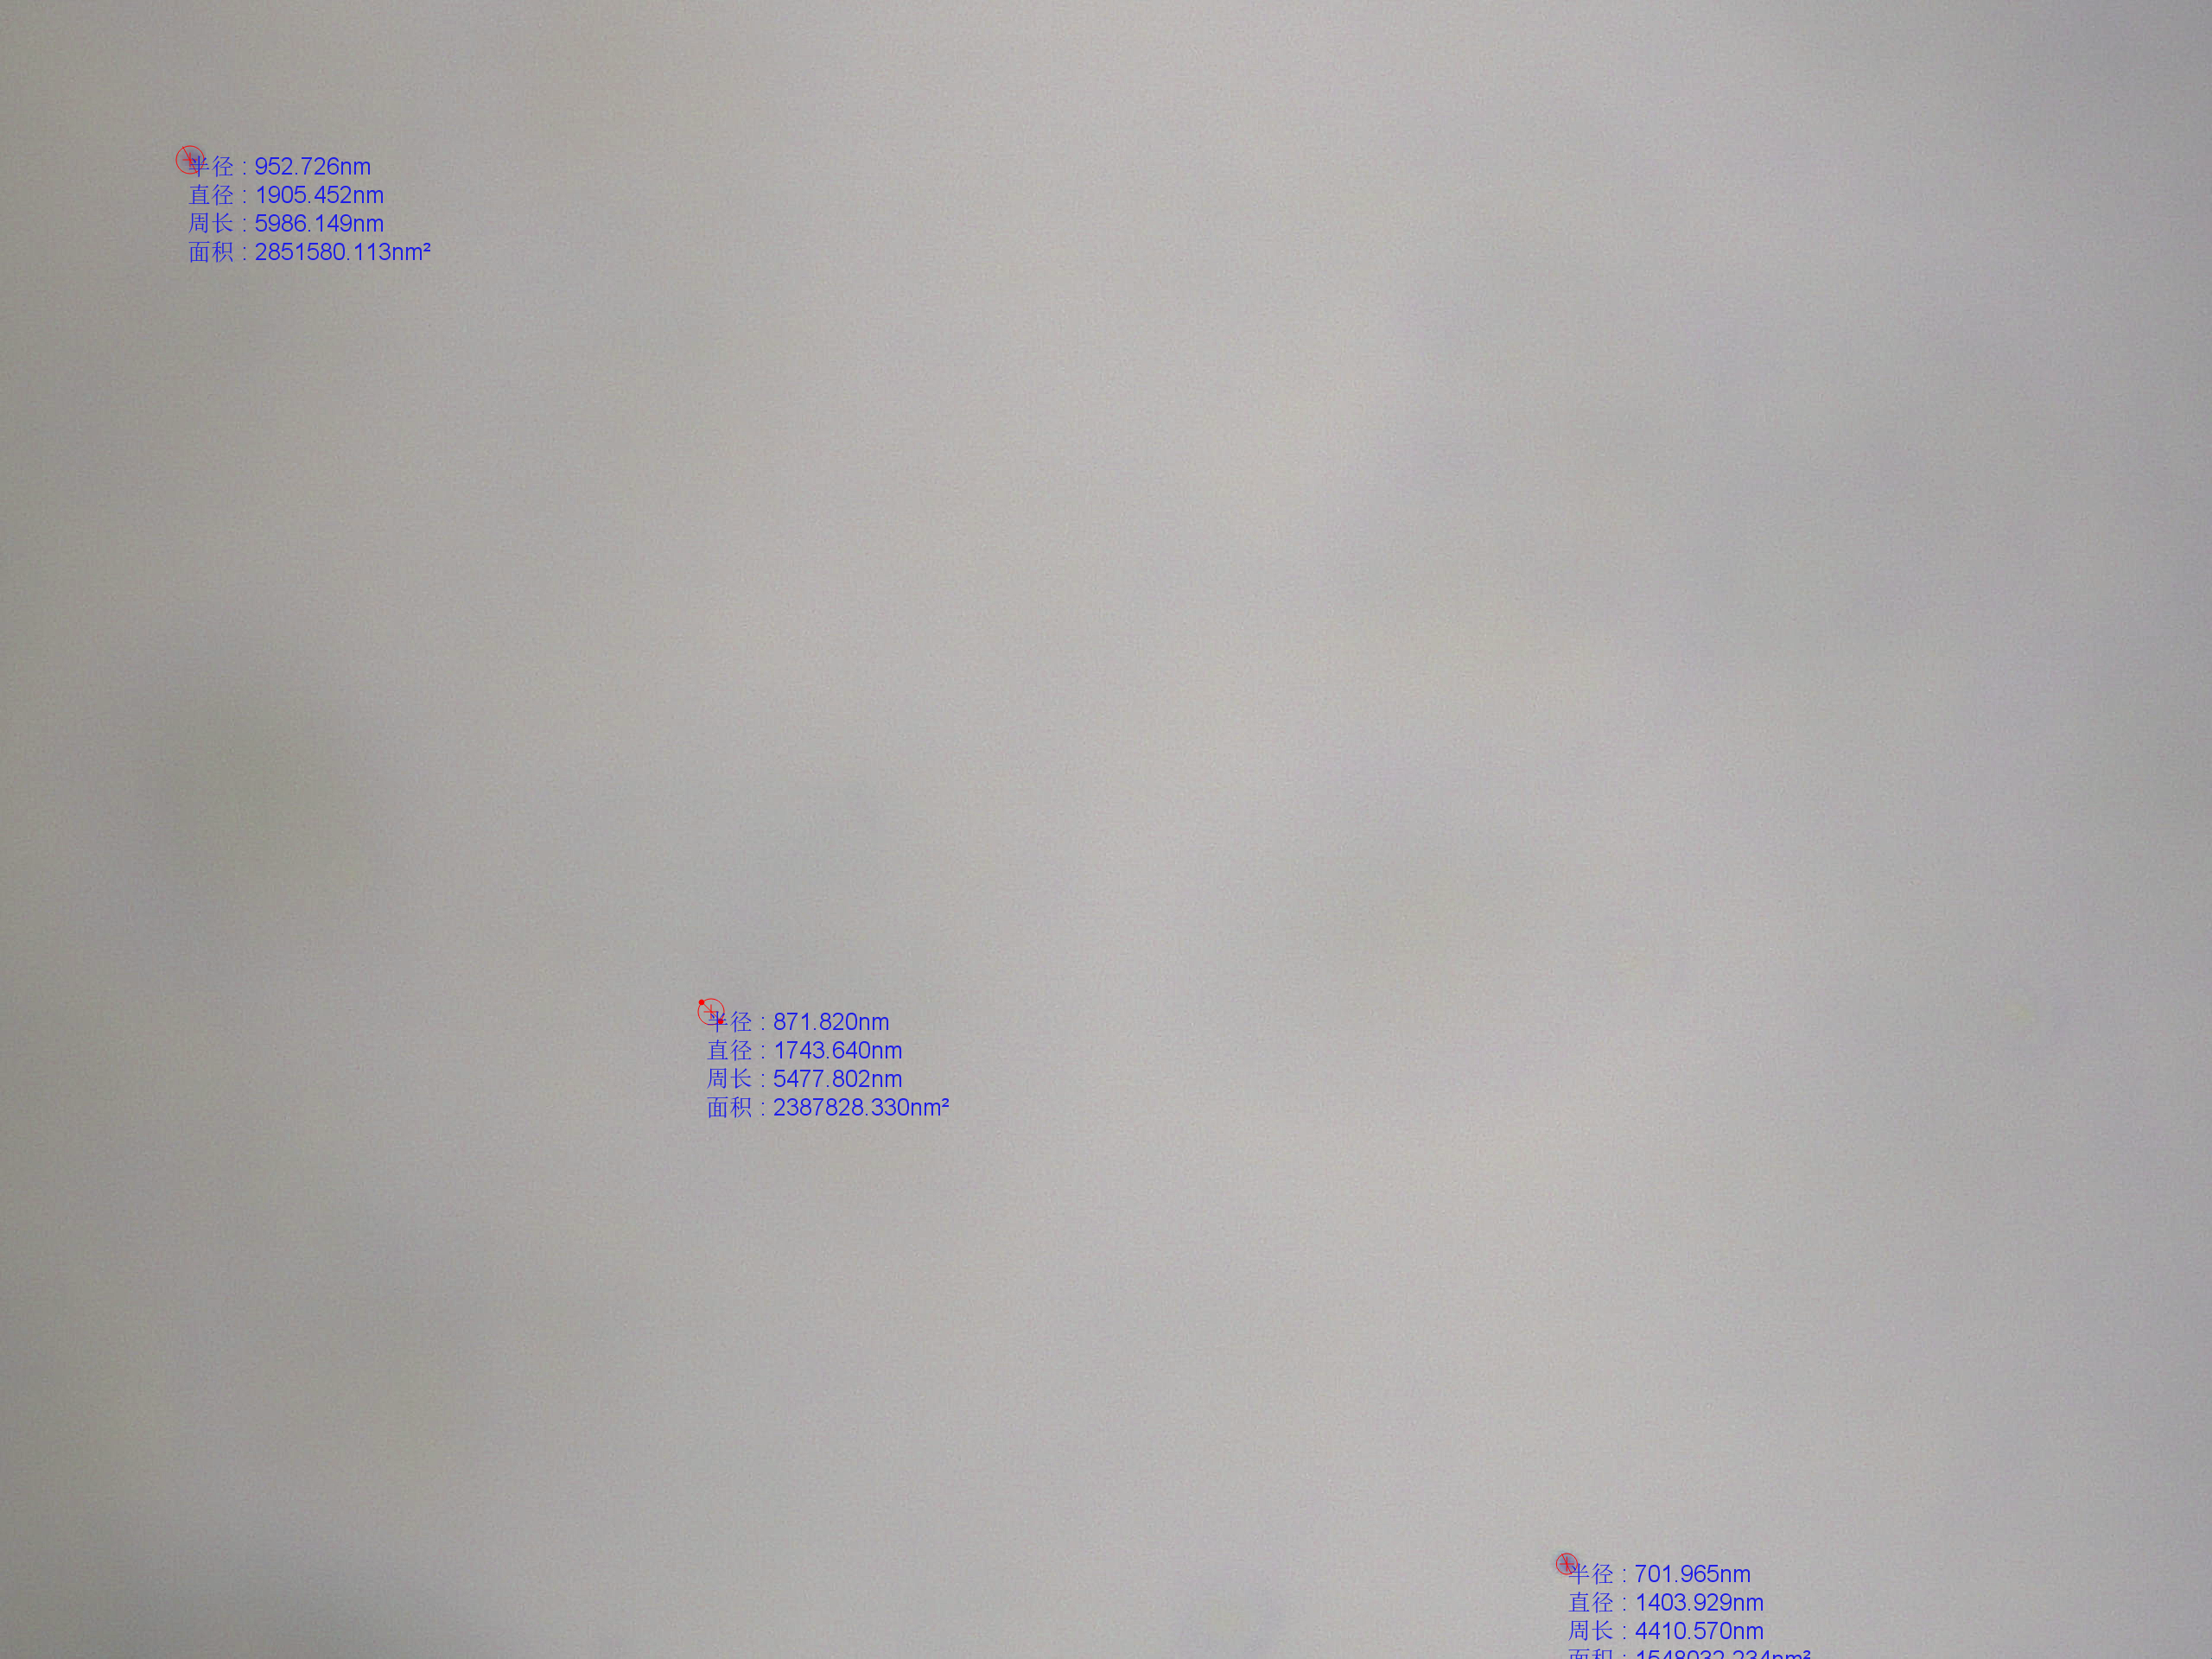
\includegraphics[width=0.65\linewidth]{src/data/1/1.png}
	\caption{{\zihaoWu 第一组样品中硫胶体粒子的显微图像}}
	\label{fig:particles}
\end{figure}

\begin{table}[htbp]
	\centering
	\caption{{\zihaoXiaoWu 各组样品硫胶体粒子的平均半径}}
	\label{tab:radius}
	\scalebox{1.2}{
		{\zihaoLiu
		\begin{tabular}{cccc}
			\toprule
			组别 & 测量粒子数 & 半径范围/nm  & 平均半径/nm \\
			\midrule
			1  & 3     & 702--953 & 842     \\
			2  & 3     & 742--957 & 856     \\
			3  & 1     & --       & 861     \\
			\bottomrule
		\end{tabular}
	}}
\end{table}

\subsection{粘度计算}

在接近室温$T$（开尔文温度）时，水的粘度$\eta_{H_2O}$可近似为：
\begin{equation}
	\eta_{H_2O} = 2.414\times10^{-5} \times 10^{\frac{247.8}{T-140}}
\end{equation}
室温23$^\circ$C（$T = 296.15$ K）时，代入公式可得$\eta_{H_2O} = 9.33\times10^{-4}$ Pa$\cdot$s。

\subsection{位移统计分析}

使用同化的数据集，计算每帧之间每个粒子的位移$\Delta x$。根据布朗运动理论，在规律的时间间隔$\tau$测量的粒子一维位移$\Delta x$的概率密度遵循高斯（正态）分布：
\begin{equation}
	P(\Delta x) = \sqrt{\frac{1}{2\pi\sigma^2}} \exp\left(-\frac{(\Delta x)^2}{2\sigma^2}\right)
\end{equation}
其中$\Delta x = x(t+\tau) - x(t)$，$\sigma = \sqrt{2D\tau}$。因此，只要数据是正态分布的，就可以根据样本数据集的标准偏差确定扩散系数$D$：
\begin{equation}
	D = \frac{\sigma^2}{2\tau}
\end{equation}

对每组数据计算时间间隔$\tau = 1$ s的位移$\Delta x$，将像素值转换为实际距离（$\mu$m）。图\ref{fig:group1}--\ref{fig:group3}分别展示了三组样品的位移直方图及正态分布拟合曲线。

\begin{figure}[htbp]
	\centering
	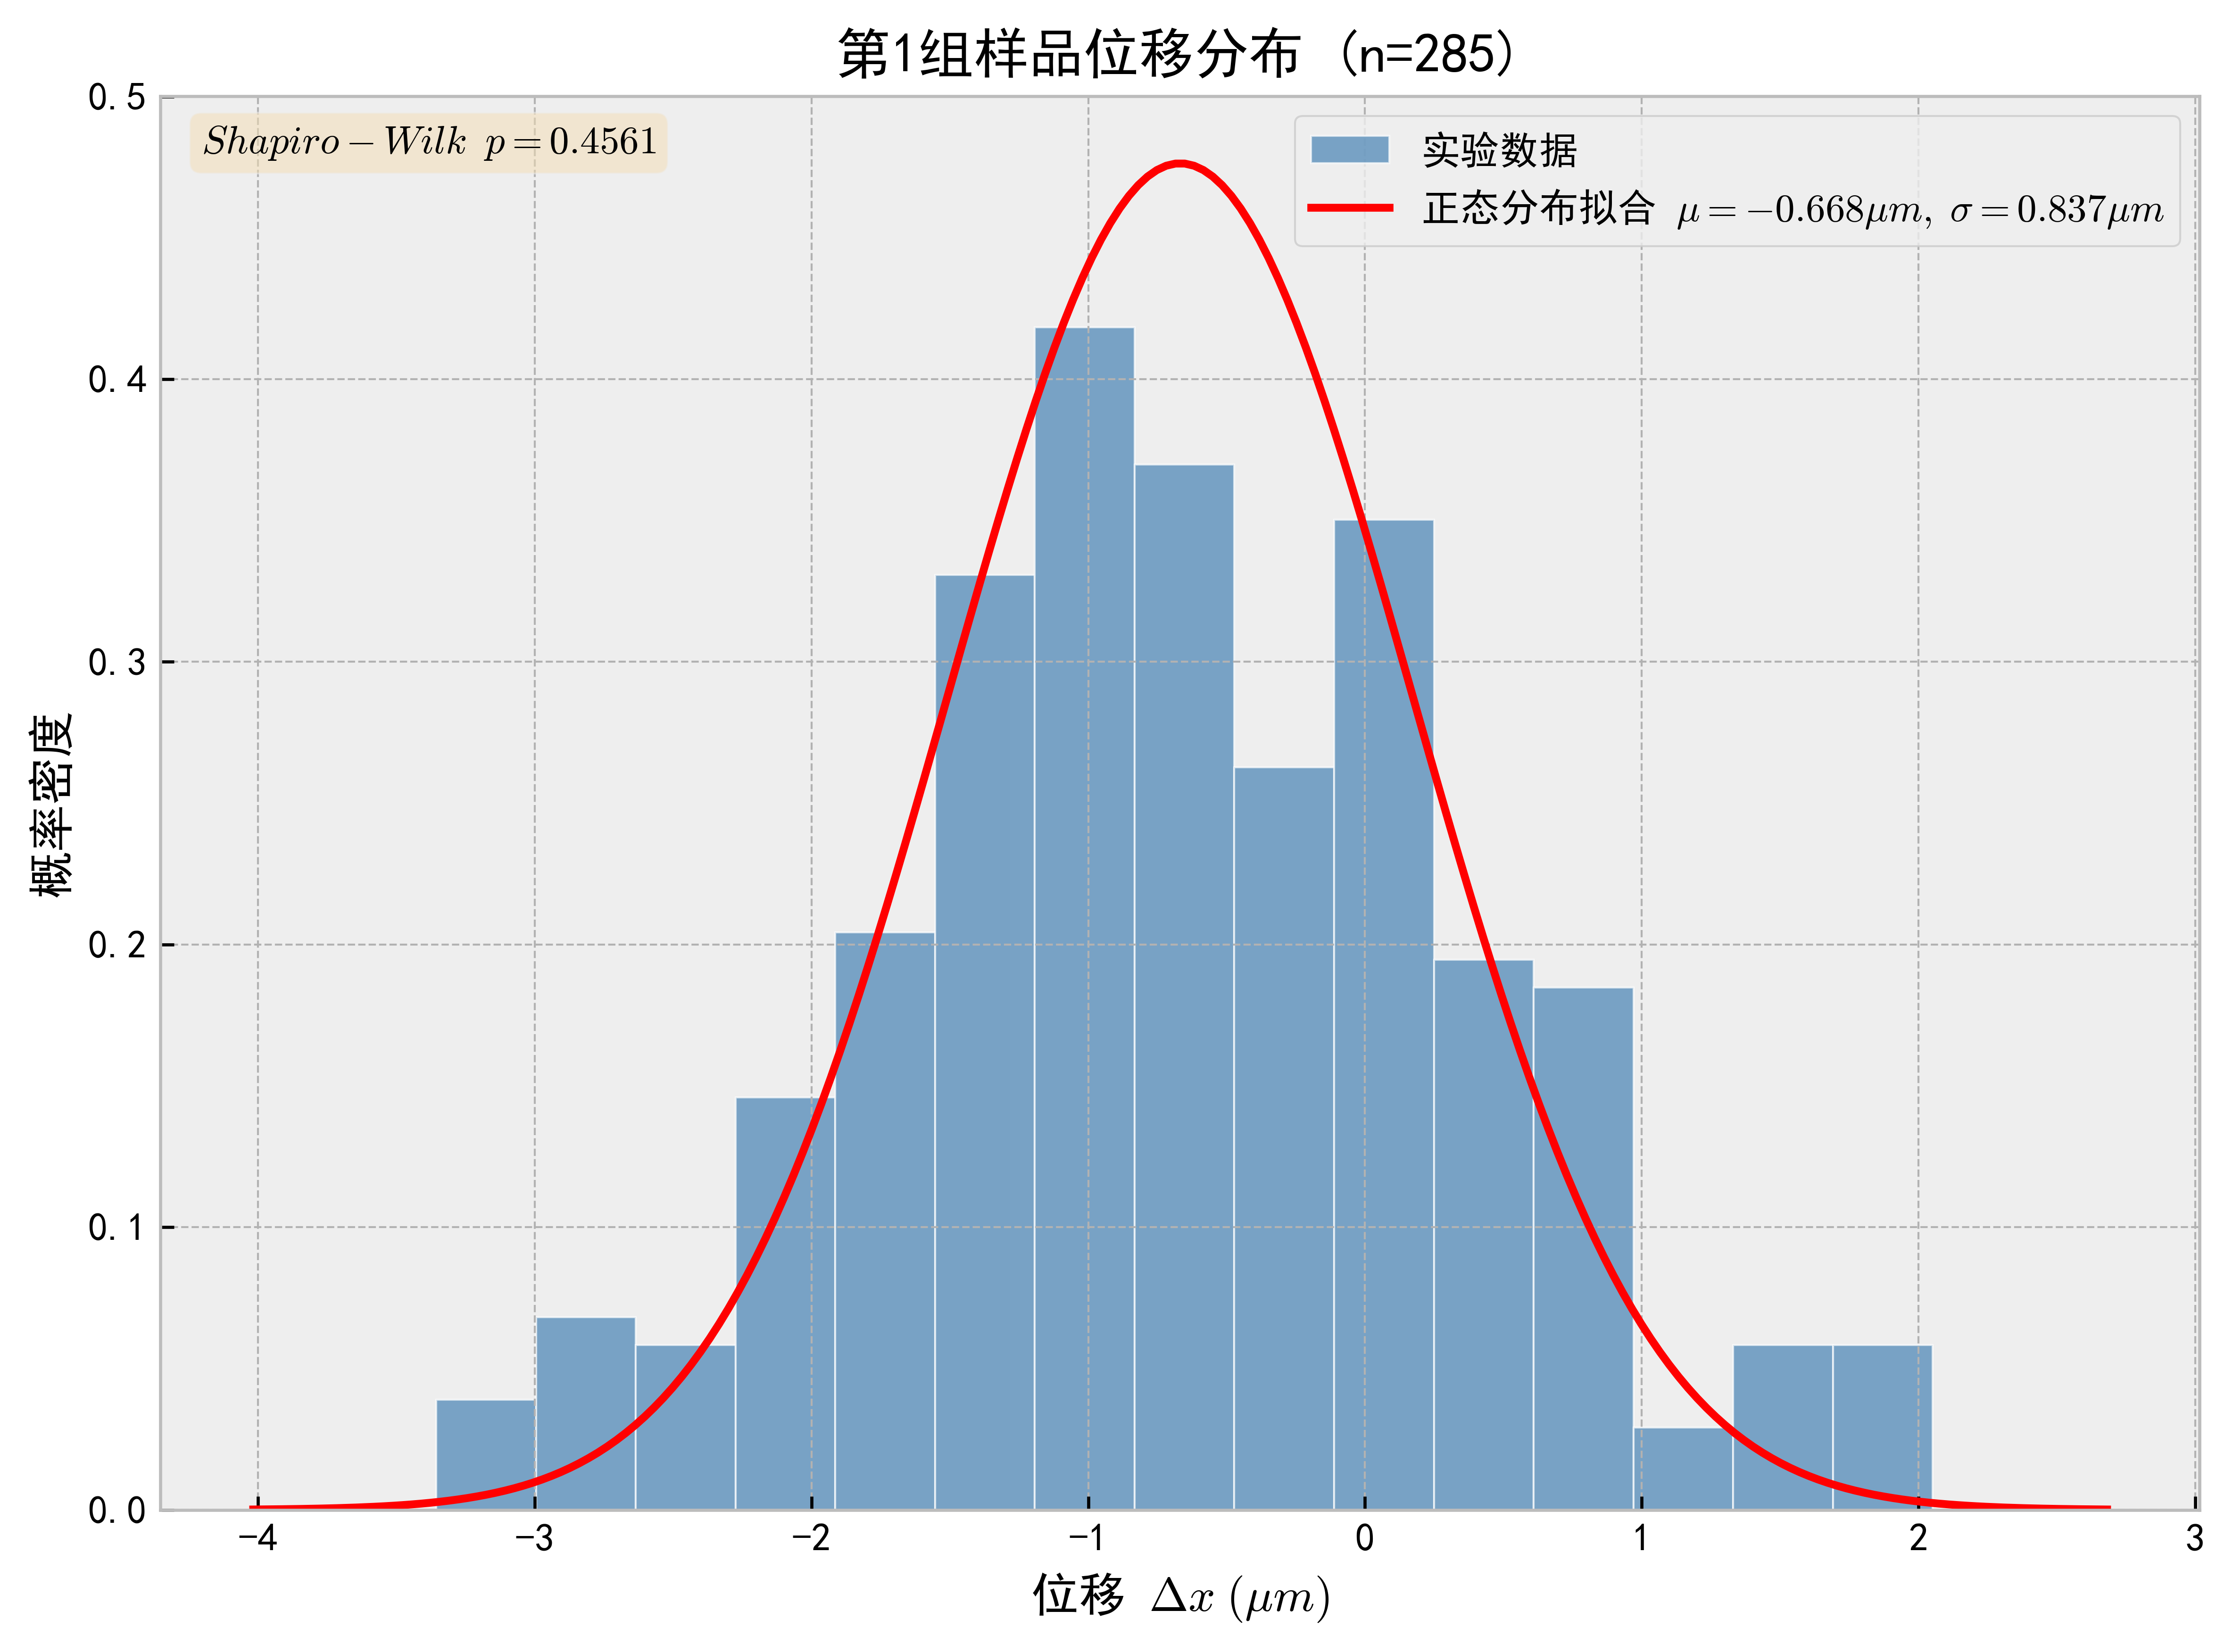
\includegraphics[width=0.85\linewidth]{src/img/group1_histogram.png}
	\caption{{\zihaoWu 第一组样品位移分布及正态拟合}}
	\label{fig:group1}
\end{figure}

\begin{figure}[htbp]
	\centering
	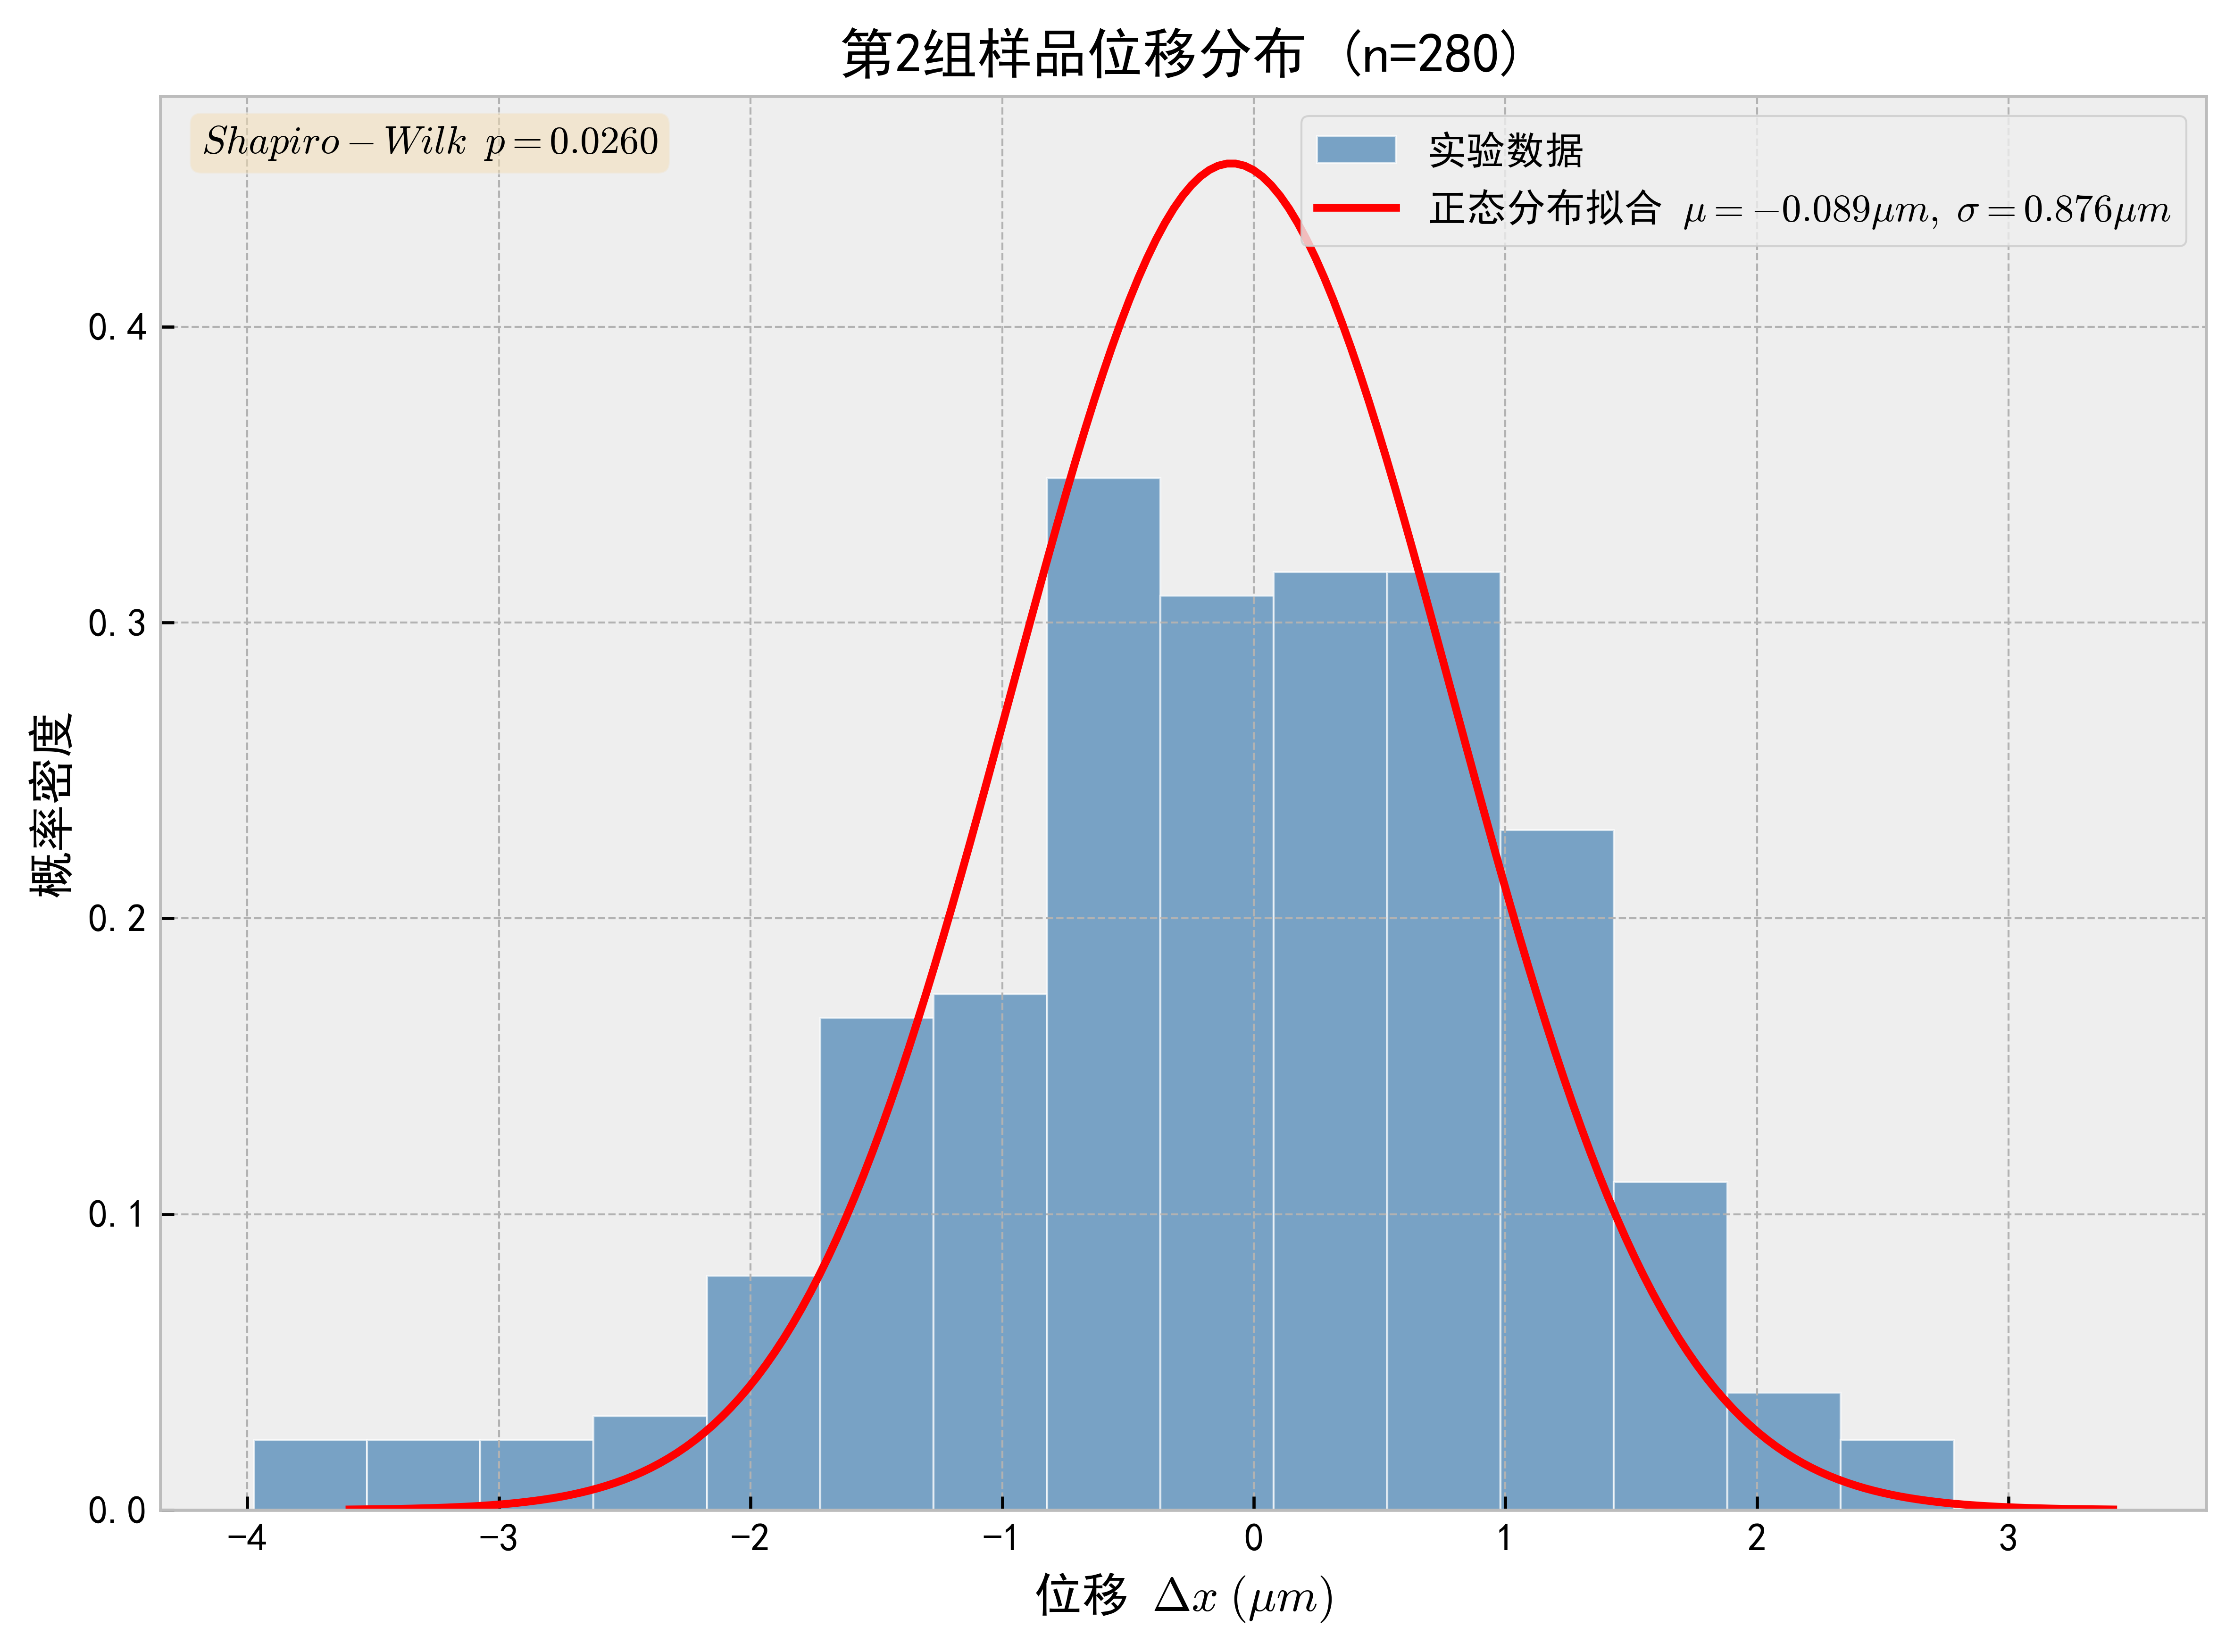
\includegraphics[width=0.85\linewidth]{src/img/group2_histogram.png}
	\caption{{\zihaoWu 第二组样品位移分布及正态拟合}}
	\label{fig:group2}
\end{figure}

\begin{figure}[htbp]
	\centering
	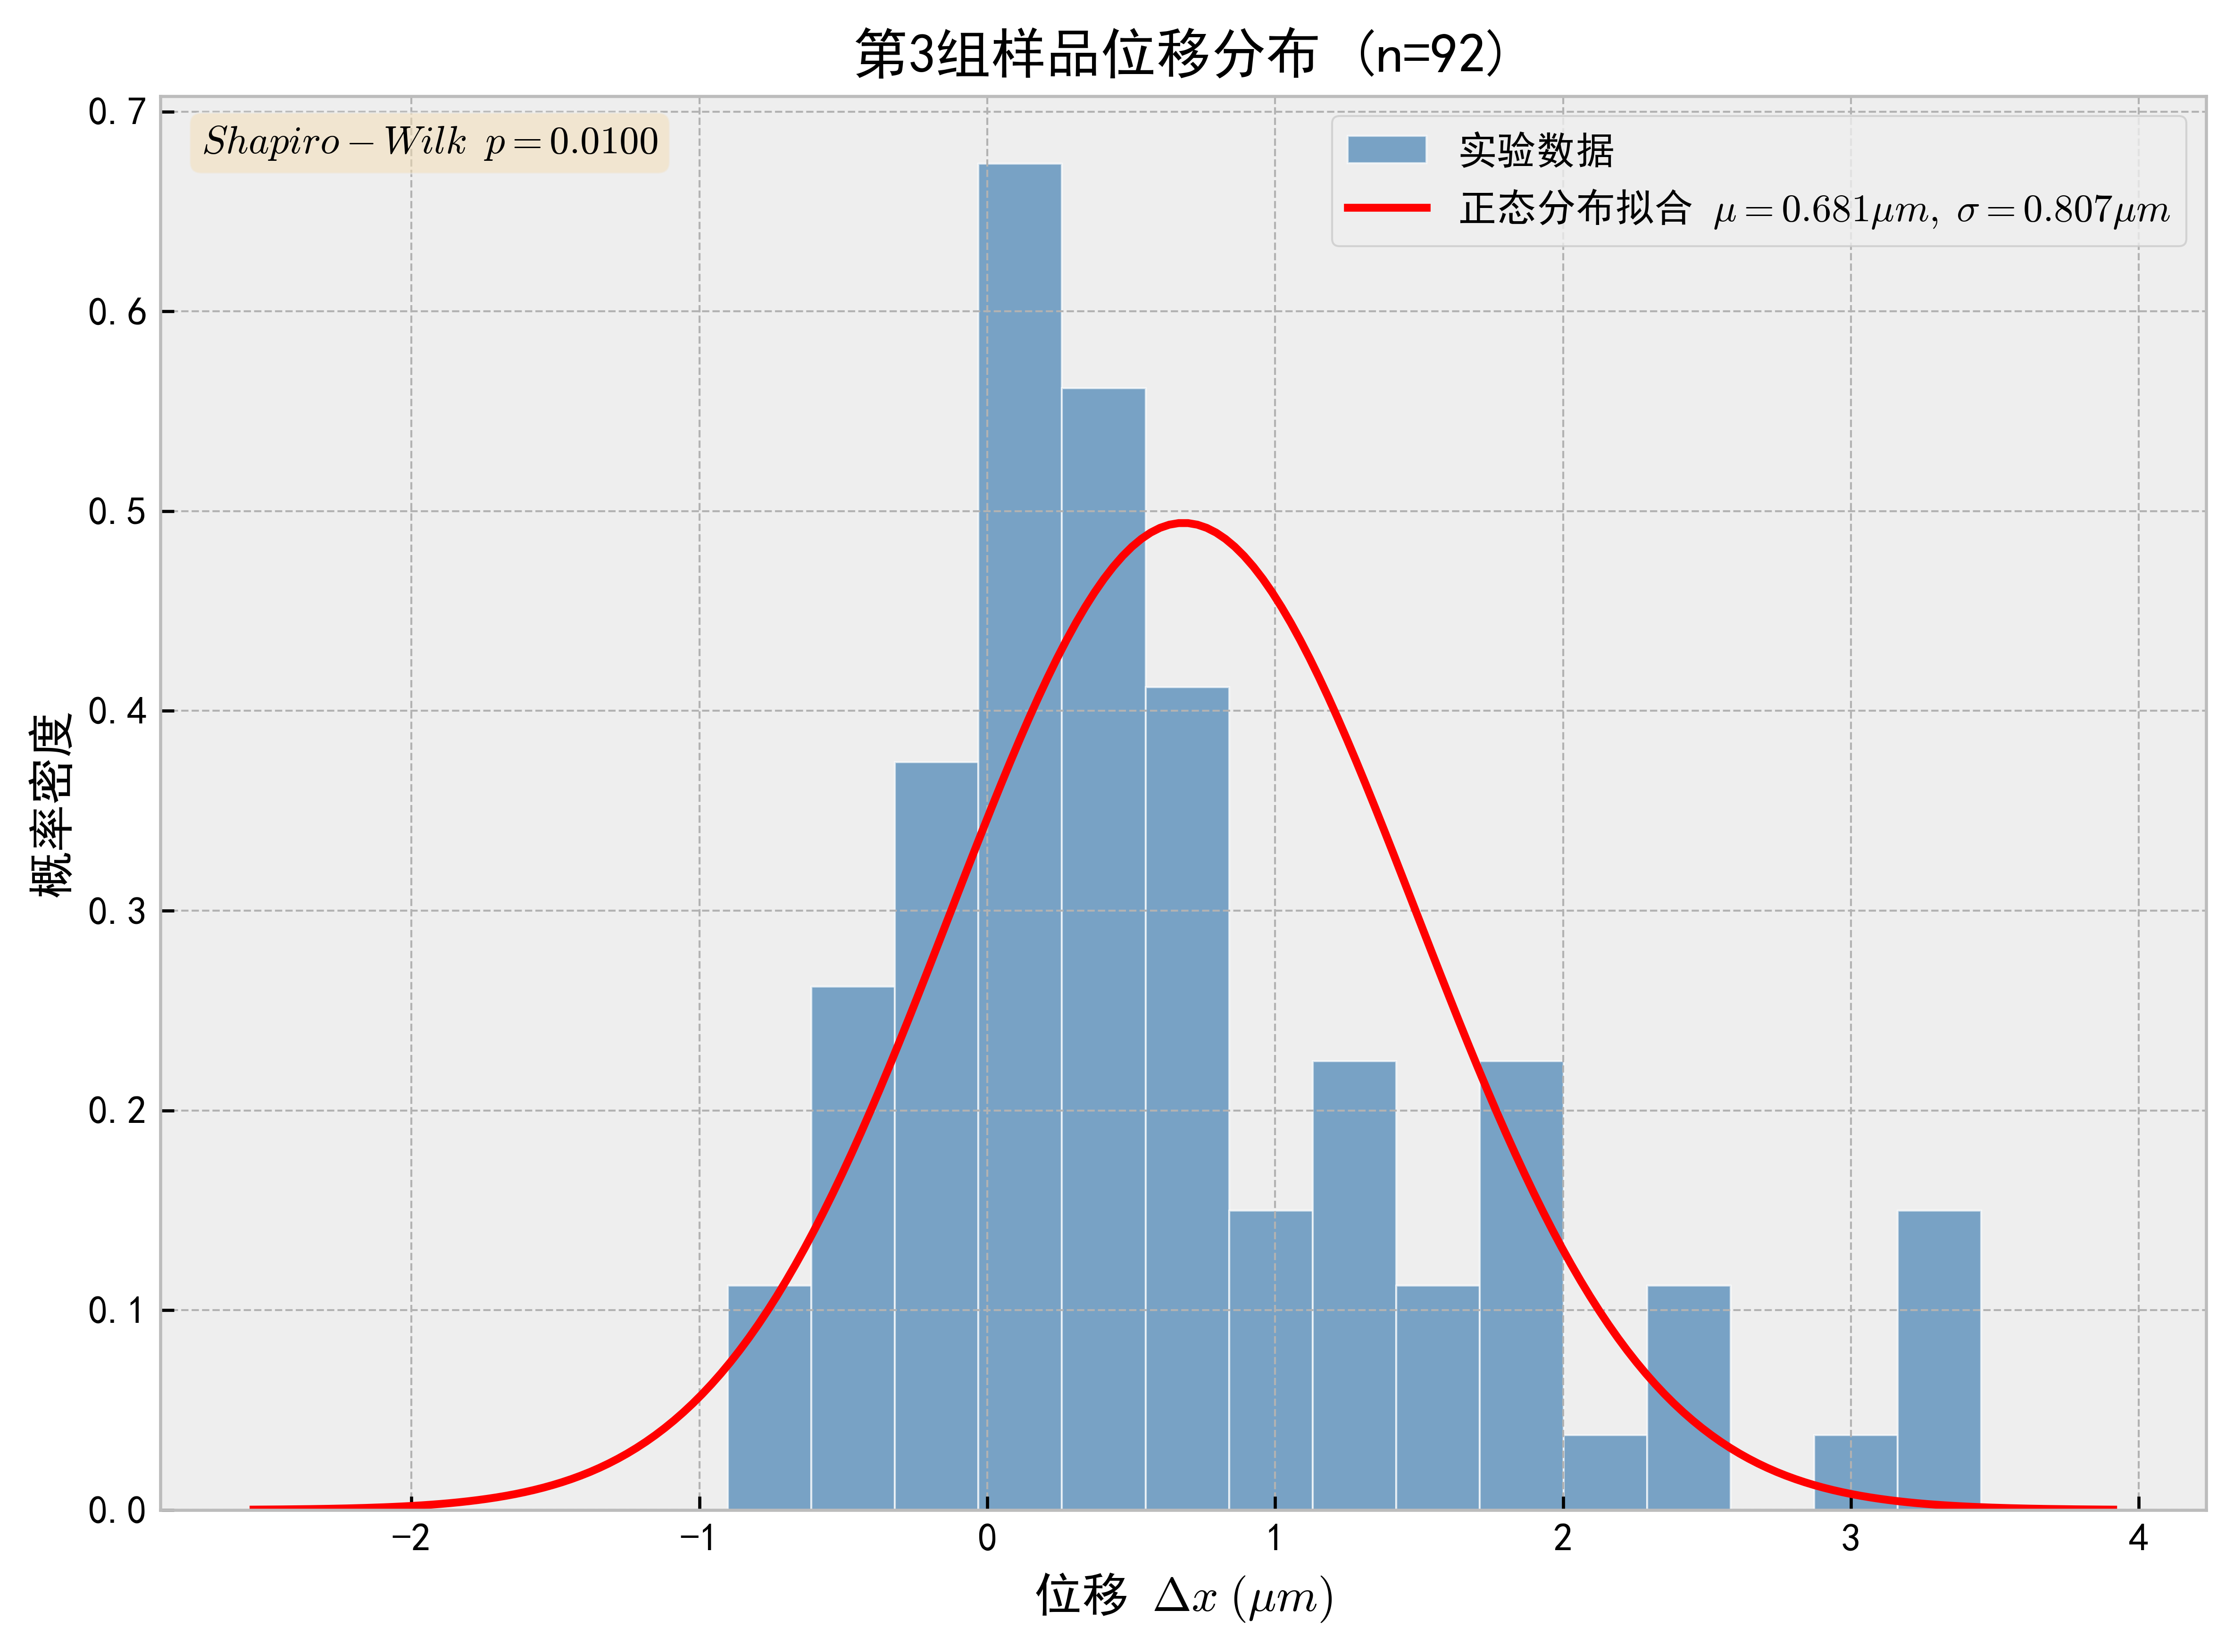
\includegraphics[width=0.85\linewidth]{src/img/group3_histogram.png}
	\caption{{\zihaoWu 第三组样品位移分布及正态拟合}}
	\label{fig:group3}
\end{figure}

各组数据的统计分析结果如表\ref{tab:stats}所示。使用Shapiro-Wilk检验对位移数据进行正态性检验。第一组数据的$p = 0.456 > 0.05$，表明位移分布符合正态分布，高斯拟合效果较好。第二组和第三组的$p$值较低（分别为0.026和0.010），可能受到极端值的影响，并且本实验的样本量很小，使用S-W检验效果可能不佳。但观察图片，正态分布效果仍在可接受范围内。

\begin{table}[htbp]
	\centering
	\caption{{\zihaoXiaoWu 各组位移统计及玻尔兹曼常数计算结果}}
	\label{tab:stats}
	\scalebox{1.2} {
	{\zihaoLiu
		\begin{tabular}{ccccccc}
			\toprule
			组别 & 样本数$n$ & 平均位移/$\mu$m & 标准差$\sigma$/$\mu$m & 扩散系数$D$/(m$^2$/s)    & $k_B$/(10$^{-23}$ J/K) & Shapiro-Wilk $p$值 \\
			\midrule
			1  & 285    & $-0.668$    & 0.837              & $3.51\times10^{-13}$ & 1.75                   & 0.456             \\
			2  & 280    & $-0.089$    & 0.876              & $3.84\times10^{-13}$ & 1.95                   & 0.026             \\
			3  & 92     & $0.681$     & 0.807              & $3.26\times10^{-13}$ & 1.67                   & 0.010             \\
			\midrule
			合计 & 657    & $-0.232$    & 0.877              & $3.85\times10^{-13}$ & 1.94                   & 0.096             \\
			\bottomrule
		\end{tabular}
	} }
\end{table}

图\ref{fig:combined}展示了所有数据合并后的位移分布。合并数据的Shapiro-Wilk检验$p$值为0.096，略高于显著性水平0.05，表明总体位移分布近似符合正态分布，验证了布朗运动的随机性特征。

\begin{figure}[htbp]
	\centering
	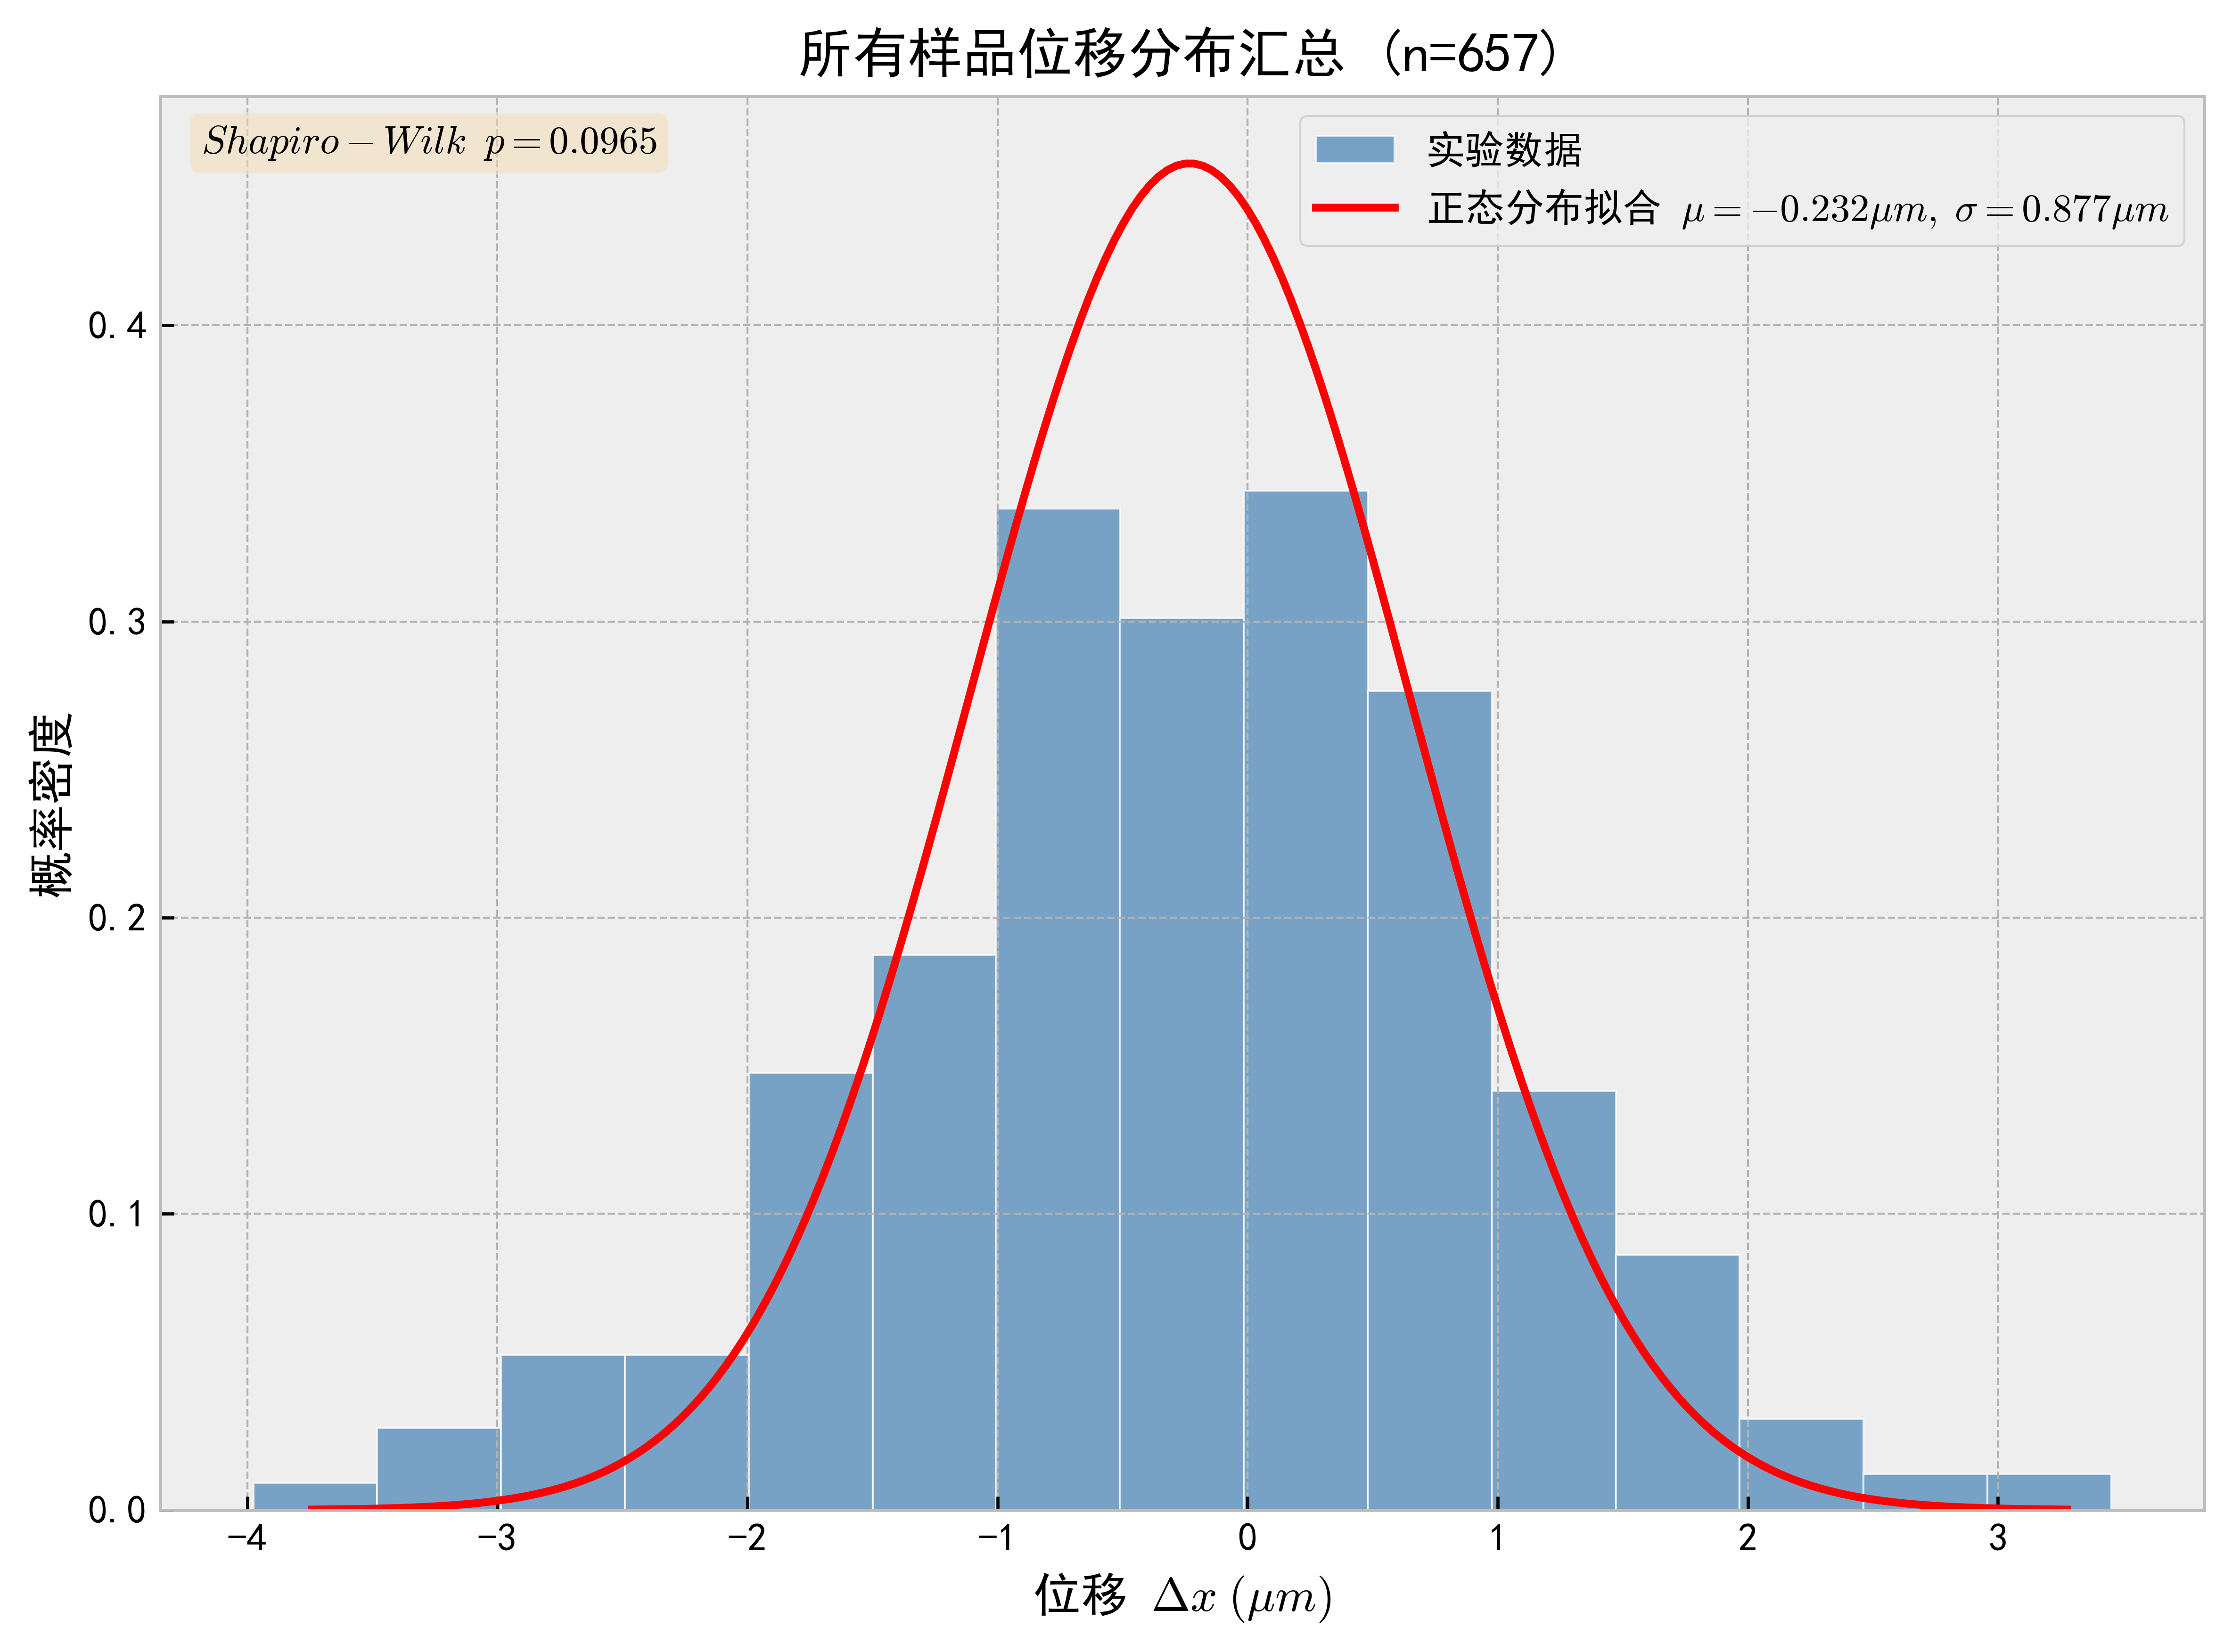
\includegraphics[width=0.85\linewidth]{src/img/combined_histogram.png}
	\caption{{\zihaoWu 所有样品位移分布汇总及正态拟合}}
	\label{fig:combined}
\end{figure}

\subsection{玻尔兹曼常数计算}

对于半径为$r$的球形胶体颗粒，阻力系数由斯托克斯定律给出：
\begin{equation}
	\varepsilon = 6\pi\eta r
\end{equation}
再根据斯托克斯-爱因斯坦方程，可求出玻尔兹曼常数：
\begin{equation}
	D = \frac{k_BT}{6\pi\eta r} \quad \Rightarrow \quad k_B = \frac{6\pi\eta rD}{T}
\end{equation}

以合并数据为例进行计算。由表\ref{tab:stats}，合并后位移的标准差$\sigma = 0.877$ $\mu$m $= 8.77\times10^{-7}$ m，时间间隔$\tau = 1$ s，因此扩散系数为：
\begin{equation}
	D = \frac{\sigma^2}{2\tau} = \frac{(8.77\times10^{-7})^2}{2\times1} = 3.85\times10^{-13} \text{ m}^2/\text{s}
\end{equation}

代入平均粒子半径$r = 851$ nm $= 8.51\times10^{-7}$ m，水的粘度$\eta = 9.33\times10^{-4}$ Pa$\cdot$s，温度$T = 296.15$ K：
\begin{equation}
	k_B = \frac{6\pi \times 9.33\times10^{-4} \times 8.51\times10^{-7} \times 3.85\times10^{-13}}{296.15} = 1.94\times10^{-23} \text{ J/K}
\end{equation}

实验测得的玻尔兹曼常数平均值为$1.94\times10^{-23}$ J/K，与标准值$1.38\times10^{-23}$ J/K相比，相对误差约41\%。实验值偏大的可能原因：

\begin{enumerate}[label=(\arabic*),leftmargin=3em]
	\item 由于显微镜的分辨率有限，粒径接近或小于光学衍射极限时，颗粒成像表现为艾里斑，导致视觉尺寸显著大于实际粒径。这一系统误差使半径测量值偏大，从而在计算中引入误差。
	\item 实验中可追踪的有效粒子数量有限，统计样本量不足，加之部分序列存在净漂移现象，使得均方位移中包含非扩散成分，影响扩散系数拟合的准确性。
	\item 硫胶体体系中残留有未反应的盐酸及反应生成的氯化钠和二氧化硫等溶质，使得实际分散介质的粘度高于纯水。在计算中使用纯水的粘度值，会使扩散系数偏低，进而影响玻尔兹曼常数的估算结果。
	\item 时间间隔的测量存在误差，实际间隔可能与设定的1秒存在偏差。
\end{enumerate}

% ======================================================
\section{思考题}
\vspace{-0.5em}

\subsection{在分子尺度上，液体的什么性质决定了它的粘度？}

粘度主要由以下因素决定：
\begin{enumerate}[label=(\arabic*),leftmargin=3em]
	\item \textbf{分子间作用力}：粘度源于流体内部的摩擦力。分子间作用力（如氢键、范德华力）越强，分子相对运动时的阻力越大，粘度越高。
	\item \textbf{分子形状与结构}：分子链越长、结构越复杂，越容易发生缠结，从而增大粘度。球形小分子则阻力较小。
	\item \textbf{动量传递}：粘度也反映了分子在不同流速层间进行动量交换的效率。
\end{enumerate}

\subsection{当$t$很大时，朗之万方程的解会发生什么变化？}

朗之万方程的解$\langle \frac{d(x^2)}{dt} \rangle = \frac{2k_BT}{\varepsilon} + Ae^{-\frac{\varepsilon t}{m}}$中，当$t$很大时，指数项$Ae^{-\frac{\varepsilon t}{m}} \rightarrow 0$。此时，描述粒子运动的方程中的惯性项可忽略，系统进入扩散主导的"过阻尼"状态。均方位移（MSD）与时间$t$呈线性关系$\langle x^2\rangle = 2Dt$，粒子的运动完全由热涨落和粘滞阻力之间的平衡所决定。

\subsection{为什么此测量需要至少1 fps的帧速率？}

准确计算玻尔兹曼常数的前提是获得可靠的扩散系数$D$，这需要验证$\langle x^2\rangle = 2Dt$的线性关系。该关系仅在时间间隔足够短、粒子运动处于正常扩散区时才严格成立。帧率过低会导致时间步长过大，丢失高频热涨落信息，引入平均误差，从而影响$D$值的准确性。本实验中帧率设置为1 fps，时间间隔$\tau = 1$ s，满足布朗运动的观测要求。

\subsection{净漂移如何影响胶体粒子的$\langle x\rangle$值？}

由温差、震动等引起的净漂移会在随机运动上叠加一个定向速度$v$。这会导致计算出的均方位移$\langle x^2\rangle$中包含一个与时间平方成正比的漂移项$(v\cdot t)^2$，使得表观扩散系数$D$偏大，最终导致估算的玻尔兹曼常数$k_B$严重偏离真实值。本实验中，第一组数据的平均位移为$-0.668$ $\mu$m，第三组为$0.681$ $\mu$m，说明可能存在一定程度的净漂移，这也是实验误差的来源之一。

\subsection{为什么要收集和分析如此大量的数据以测算玻尔兹曼常数？}

\begin{enumerate}[label=(\arabic*),leftmargin=3em]
	\item \textbf{克服随机性}：布朗运动具有高度随机性。只有通过大量粒子（系综平均）或单个粒子的长时间观测（时间平均），才能使统计规律显现，从噪声中提取出有效信号。
	\item \textbf{降低不确定性}：依据大数定律，增加样本量可以减小统计误差和偶然因素（如图像识别误差、瞬时扰动）的影响，提高测量信噪比。
	\item \textbf{筛选有效数据}：大量数据有助于识别并剔除受边界效应、粒子团聚或杂质干扰的异常轨迹。
	\item \textbf{保证精度}：玻尔兹曼常数是一个微观基本常数，对测量误差极为敏感。庞大的数据集是获得可靠、高精度实验结果的必要前提。
\end{enumerate}

本实验共采集657个有效位移数据点（第一组285个，第二组280个，第三组92个），通过合并分析提高了统计可靠性。

\subsection{GFP分子在细胞中的扩散时间计算及对细胞转运机制的启示}

已知绿色荧光蛋白（GFP）的扩散系数$D = 30$ $\mu$m$^2$/s。在三维中，粒子的均方位移由$\langle R^2\rangle = 6Dt$给出。对于直径约20 $\mu$m的细胞，$\langle R^2\rangle = 400$ $\mu$m$^2$，根据扩散公式：
\begin{equation}
	t = \frac{\langle R^2\rangle}{6D} = \frac{400}{6\times30} \approx 2.22 \text{ s}
\end{equation}

这表明对于直径约20 $\mu$m的细胞，像GFP这样的蛋白质分子只需约2秒即可通过扩散遍布整个细胞，说明对于小尺度空间，扩散是一种高效的输运方式。

然而，当细胞尺度扩大10倍（至200 $\mu$m）时，$\langle R^2\rangle$增加100倍，扩散时间将激增至约222秒（约4分钟）。这表明对于大型细胞或长距离运输（如神经轴突运输），必须依赖消耗ATP的主动运输机制才能满足生理需求。

\vspace{1em}
\noindent\textbf{实验后思考题}
\vspace{0.5em}

\subsection{数据筛选与同化}

对于采集的粒子位置数据，首先需要删除图像捕获过程中未成功跟踪的粒子对应的所有数据（如Tracker软件中标记为Missing的条目）。这种情况表示在分析过程中粒子失去了轨迹，例如粒子移出显微镜的焦平面。对三组数据集采取同样的操作，并将剩余的有用数据同化在单独的电子表格中。本实验中，经过筛选后共保留657个有效位移数据点。

\subsection{位移直方图与扩散系数计算}

使用同化的数据集，计算每帧之间每个粒子的位移$\Delta x = x(t+\tau) - x(t)$，其中$\tau = 1$ s。绘制所有$\Delta x$值的直方图，以确定位移是否呈正态分布。

本实验结果显示，合并后的位移数据通过Shapiro-Wilk正态性检验（$p = 0.096 > 0.05$），表明位移分布符合正态分布。位移的标准偏差$\sigma = 0.877$ $\mu$m $= 8.77\times10^{-7}$ m，将距离单位从像素转换为米后，扩散系数为：
\begin{equation}
	D = \frac{\sigma^2}{2\tau} = \frac{(8.77\times10^{-7})^2}{2\times1} = 3.85\times10^{-13} \text{ m}^2/\text{s}
\end{equation}

\subsection{不同时间间隔的位移直方图比较}

对于$\tau = 2$ s或$\tau = 3$ s时的位移直方图，与$\tau = 1$ s相比会有以下差异：

\begin{enumerate}[label=(\arabic*),leftmargin=3em]
	\item \textbf{分布变宽}：根据$\sigma = \sqrt{2D\tau}$，时间间隔增大时标准偏差增大，直方图的宽度变宽。
	\item \textbf{峰值降低}：由于概率密度归一化，分布变宽后峰值相应降低。
	\item \textbf{仍保持正态分布}：只要粒子处于正常扩散状态，位移分布仍服从高斯分布。
\end{enumerate}

图\ref{fig:tau_compare}展示了三种时间间隔下的位移分布对比。实验结果表明，随着$\tau$增大，分布确实变宽，且标准偏差的变化符合$\sigma \propto \sqrt{\tau}$的理论预期：$\tau = 1$ s时$\sigma_1 \approx 0.877$ μm，$\tau = 2$ s时$\sigma_2 \approx 1.24$ μm $\approx \sqrt{2}\sigma_1$，$\tau = 3$ s时$\sigma_3 \approx 1.52$ μm $\approx \sqrt{3}\sigma_1$。

\begin{figure}[htbp]
	\centering
	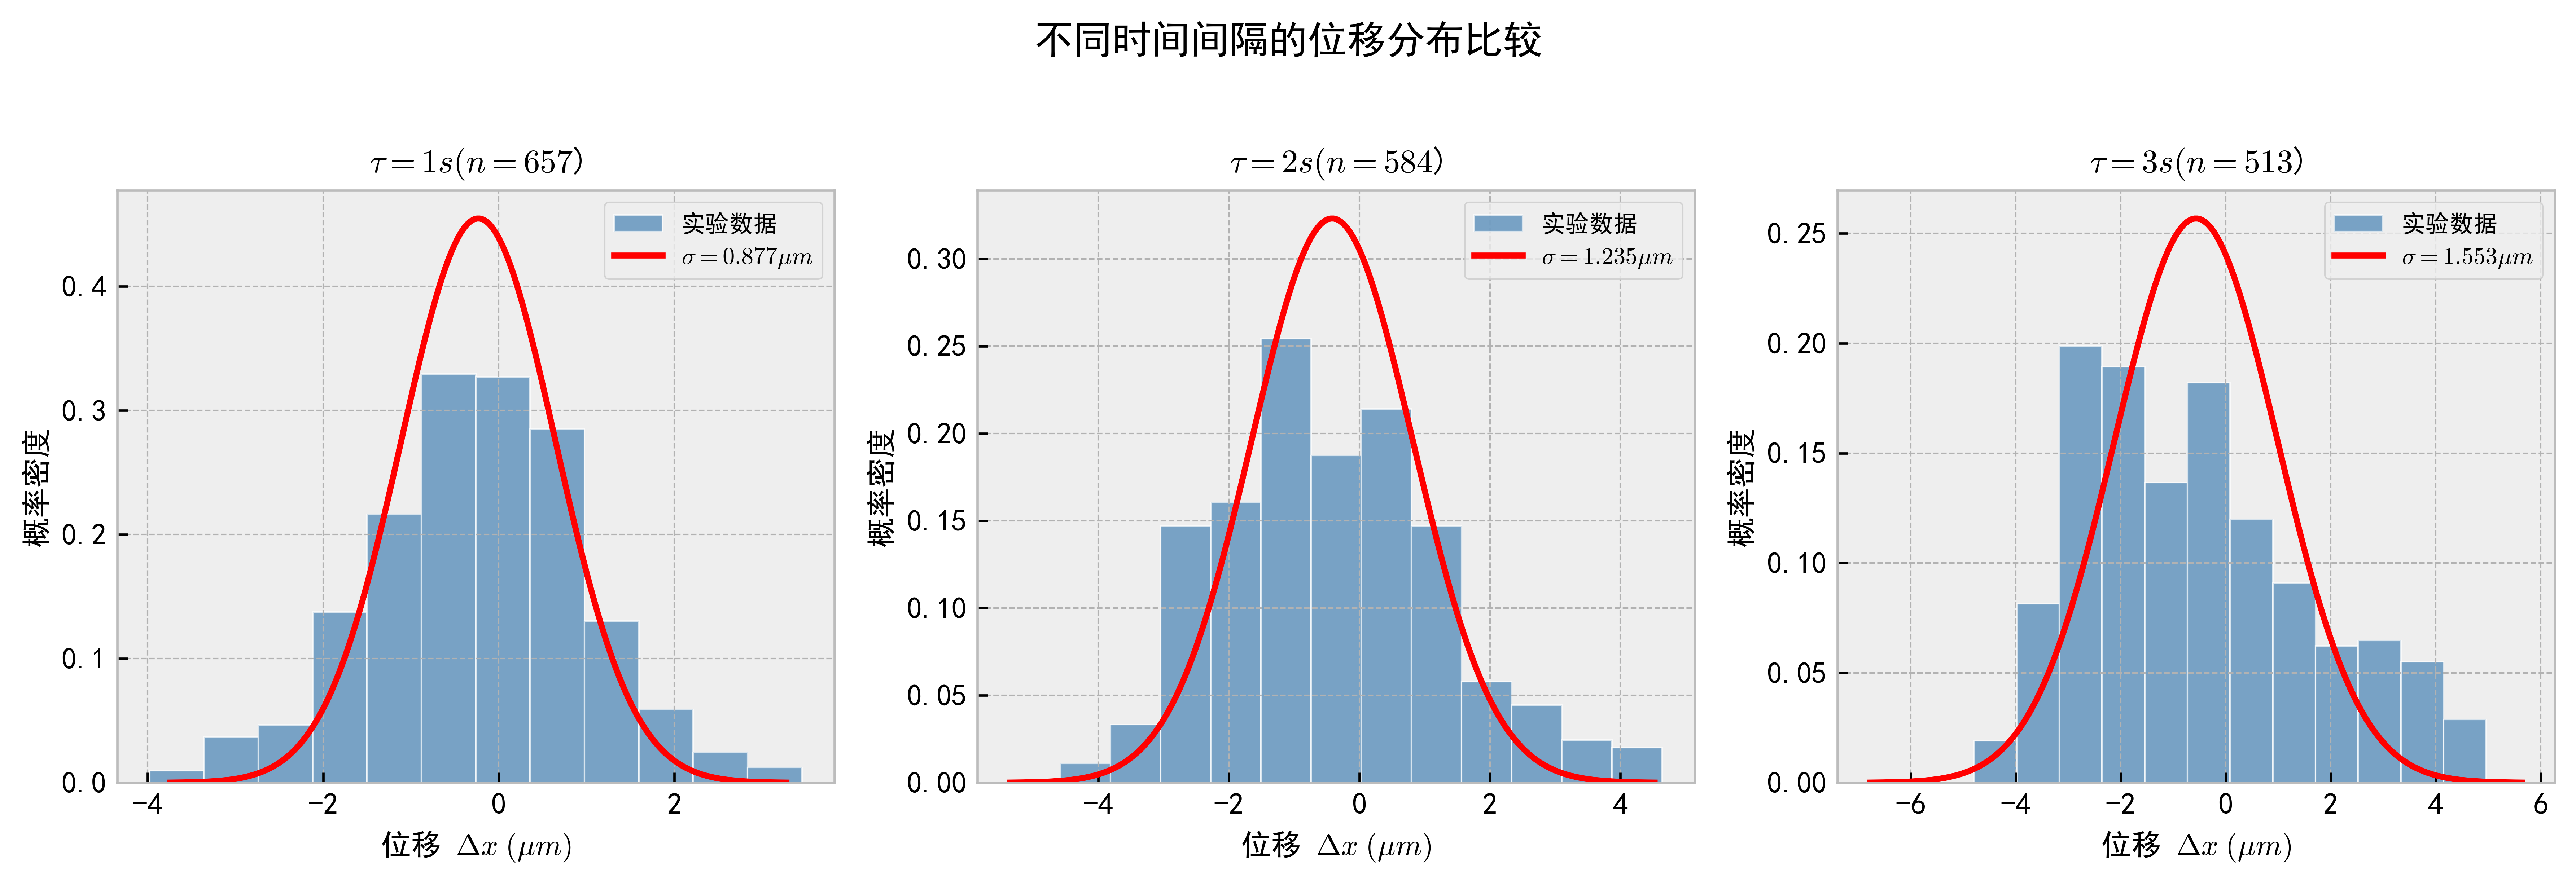
\includegraphics[width=0.95\linewidth]{src/img/displacement_comparison.png}
	\caption{{\zihaoWu 不同时间间隔下的位移分布比较}}
	\label{fig:tau_compare}
\end{figure}

\subsection{玻尔兹曼常数计算}

使用实验温度$T = 296.15$ K和估算的硫粒子平均半径$r = 851$ nm，根据斯托克斯-爱因斯坦方程计算玻尔兹曼常数：
\begin{equation}
	k_B = \frac{6\pi\eta rD}{T} = \frac{6\pi \times 9.33\times10^{-4} \times 8.51\times10^{-7} \times 3.85\times10^{-13}}{296.15} = 1.94\times10^{-23} \text{ J/K}
\end{equation}

与标准值$k_B = 1.38\times10^{-23}$ J/K相比，相对误差约为41\%。

\subsection{均方位移与线性回归}

将所有$x$和$y$跟踪坐标同化到单个文档中，过滤掉跟踪过程中丢失的粒子。对于每个粒子，计算相对于初始位置的平方位移：
\begin{equation}
	R(t)^2 = (x(t) - x(0))^2 + (y(t) - y(0))^2
\end{equation}

由此计算每个时间点的均方位移$\langle R(t)^2 \rangle$。对于在二维平面中移动的粒子，均方位移与时间的关系为：
\begin{equation}
	\langle R(t)^2 \rangle = 4Dt
\end{equation}

图\ref{fig:msd}展示了实验测得的均方位移与时间的关系。数据点呈现出良好的线性关系，符合正常扩散的理论预期。

\begin{figure}[htbp]
	\centering
	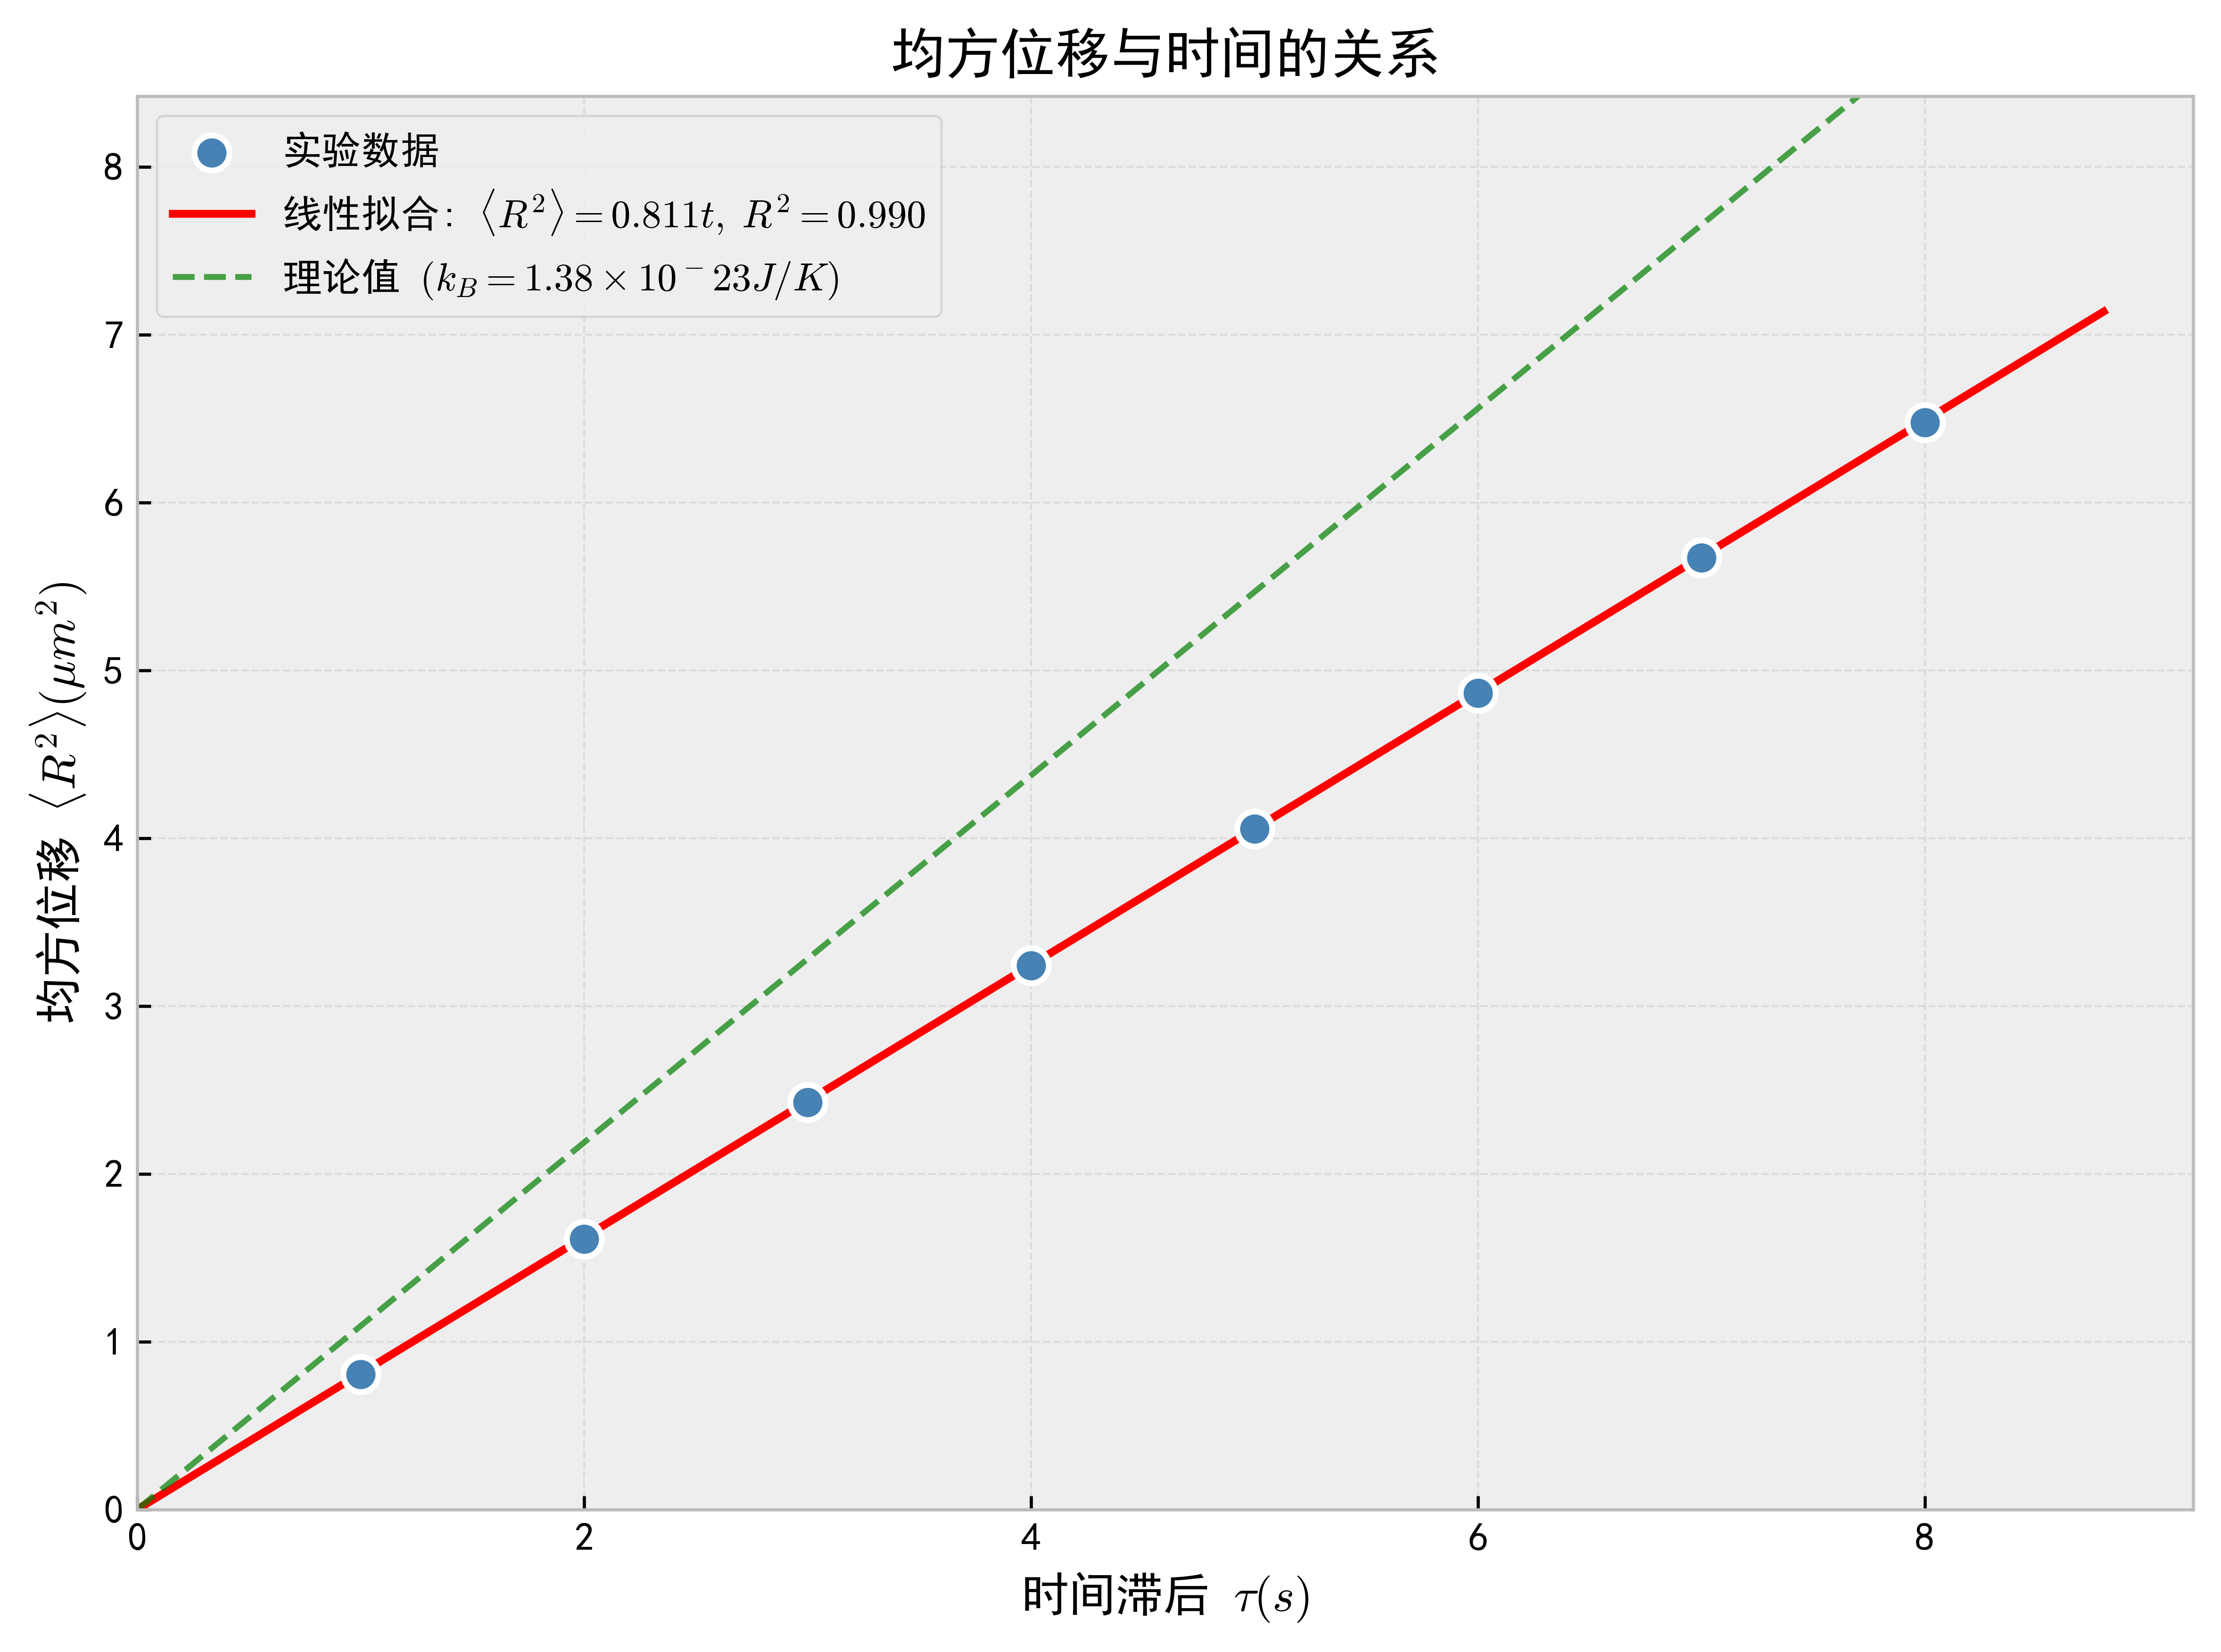
\includegraphics[width=0.85\linewidth]{src/img/msd_vs_time.png}
	\caption{{\zihaoWu 均方位移与时间的线性关系}}
	\label{fig:msd}
\end{figure}

\subsection{线性回归法确定扩散系数}

使用线性回归拟合$\langle R(t)^2 \rangle$与$t$的关系，从斜率可以得到扩散系数$D = \text{slope}/4$。

拟合结果如表\ref{tab:msd}所示。线性回归的决定系数$R^2 = 0.990$，表明数据与线性模型高度吻合，验证了粒子处于正常扩散状态。

\begin{table}[htbp]
	\centering
	\caption{{\zihaoXiaoWu 均方位移线性回归分析结果}}
	\label{tab:msd}
	\scalebox{1.2}{
	{\zihaoLiu
		\begin{tabular}{cccccc}
			\toprule
			时间$t$/s & $\langle R^2 \rangle$/μm$^2$ & 斜率/(μm$^2$/s)          & $D$/(m$^2$/s)                         & $k_B$/(10$^{-23}$ J/K) & $R^2$                  \\
			\midrule
			1       & 0.805                        & \multirow{8}{*}{0.811} & \multirow{8}{*}{$2.03\times10^{-13}$} & \multirow{8}{*}{1.02}  & \multirow{8}{*}{0.990} \\
			2       & 1.613                        &                        &                                       &                        &                        \\
			3       & 2.427                        &                        &                                       &                        &                        \\
			4       & 3.242                        &                        &                                       &                        &                        \\
			5       & 4.057                        &                        &                                       &                        &                        \\
			6       & 4.866                        &                        &                                       &                        &                        \\
			7       & 5.673                        &                        &                                       &                        &                        \\
			8       & 6.479                        &                        &                                       &                        &                        \\
			\bottomrule
		\end{tabular}
	}}
\end{table}

由斜率计算扩散系数：
\begin{equation}
	D = \frac{\text{slope}}{4} = \frac{0.811}{4} = 0.203 \text{ μm}^2/\text{s} = 2.03\times10^{-13} \text{ m}^2/\text{s}
\end{equation}

进而计算玻尔兹曼常数：
\begin{equation}
	k_B = \frac{6\pi\eta rD}{T} = \frac{6\pi \times 9.33\times10^{-4} \times 8.51\times10^{-7} \times 2.03\times10^{-13}}{296.15} = 1.02\times10^{-23} \text{ J/K}
\end{equation}

与标准值$k_B = 1.38\times10^{-23}$ J/K相比，相对误差约为26\%，优于标准偏差法的41\%误差。

与标准偏差法相比，线性回归法的优势在于：
\begin{enumerate}[label=(\arabic*),leftmargin=3em]
	\item 利用了所有时间点的信息，而非仅使用单一时间间隔；
	\item 可以通过拟合优度（$R^2$值）评估数据质量；
	\item 能够检测是否存在异常扩散行为（如受限扩散或超扩散）。
\end{enumerate}

两种方法得到的玻尔兹曼常数量级一致，但线性回归法的结果更接近标准值，具有更高的统计可靠性。$R^2 = 0.990 > 0.95$表明拟合良好，数据符合正常扩散模型。

\clearpage

% ======================================================
\section{结论}
\vspace{-0.5em}

本实验成功制备出硫胶体悬浮体系，并清晰观察到微粒的布朗运动。通过对三组独立采集的数据进行一维位移的高斯拟合分析，验证了布朗运动位移服从正态分布。实验共获得657个有效位移数据点，其中第一组数据通过Shapiro-Wilk正态性检验（$p = 0.456$），表明位移分布符合理论预期。

根据扩散系数公式$D = \sigma^2/(2\tau)$和斯托克斯-爱因斯坦方程$k_B = 6\pi\eta rD/T$，实验测得的玻尔兹曼常数为$1.94\times10^{-23}$ J/K。与理论值（$1.38\times10^{-23}$ J/K）相比，相对误差约41\%，数量级一致，表明实验方法可靠。

误差主要来源于：(1) 光学显微镜分辨率限制导致的粒径测量系统误差；(2) 样本量相对有限带来的统计误差；(3) 溶液组成对粘度的影响；(4) 图像采集过程中可能存在的漂移现象。

后续研究可通过以下方式进一步提高测量精度：扩大样本量、使用更高分辨率的显微系统、优化图像识别算法、严格控制溶液组成以及确保实验环境的稳定性。

\vspace{3em}
% ======================================================
% 参考文献
{\footnotesize
	\setstretch{1}
	\begin{thebibliography}{9}
		\bibitem{einstein1905}
		Einstein A.
		\textit{Annalen der Physik}, \textbf{1905}, 322(8): 549--560

		\bibitem{perrin1909}
		Perrin J.
		\textit{Annales de Chimie et de Physique}, \textbf{1909}, 18: 5--114

		\bibitem{langevin1908}
		Langevin P.
		\textit{Comptes Rendus}, \textbf{1908}, 146: 530--533

		\bibitem{berg1993}
		Berg H C.
			{\kaishu Random Walks in Biology}.
		Princeton University Press, 1993

		\bibitem{xmu2024}
		厦门大学化学国家级实验教学示范中心.
		{\kaishu 中心科学实验IV实验讲义}.
		厦门: 厦门大学出版社, 2024
	\end{thebibliography}
}

% ======================================================
% 评语与签字栏

\vspace*{\fill}
\noindent{\zihaoWu 评语（Remarks）：}

\vspace{2em}

\begin{center}
	{\zihaoWu\bfseries 指导教师（Instructor）\hspace{8em} 日期（Date）}
\end{center}

\vspace{1.5cm}

\end{document}
